%% =====================================================================
%%  2026-11-18-問い2の提案：問い 2 の提案（感情ごとの信頼度の表で声・顔・言葉の答えをまとめる）だけを説明する資料（日本語だけ）．第 1 版
%%  研究者の依頼（2026-11-18）：「問２の提案について，高校生でもわかるように教えてください．」の会話の説明を入れ，
%%  「１２個の重みをどう使うか，何の重みか．・ｄをどう使うか．・妥当な比較手法は？・結果の絶対値（差ではなく）」に答える．
%%  範囲は「問い 2 だけの短い資料」（研究者の回答）．
%%  数値は figures/numbers.tex から \N{key} で引く（scripts/export_figdata.py が結果ファイルから書く．手で数を書かない）．
%%  模式図は 2026-11-16-共同研究者向け説明/figures/ から写した（作った台本は DAI/paper/scripts/make_figs_explain.py ほか）．
%% =====================================================================
\input{preamble}
\input{merda}
% scripts/export_figdata.py が書いた．手で直さない．
\expandafter\gdef\csname NUM@aFeightAFEWfive\endcsname{74.30}
\expandafter\gdef\csname NUM@aFeightAFEWonezero\endcsname{74.84}
\expandafter\gdef\csname NUM@aFeightAFEWtwentyfive\endcsname{76.31}
\expandafter\gdef\csname NUM@aFeightCREMADfive\endcsname{85.26}
\expandafter\gdef\csname NUM@aFeightCREMADonezero\endcsname{86.04}
\expandafter\gdef\csname NUM@aFeightCREMADtwentyfive\endcsname{87.55}
\expandafter\gdef\csname NUM@aFeightIEMOCAPfive\endcsname{71.69}
\expandafter\gdef\csname NUM@aFeightIEMOCAPonezero\endcsname{73.16}
\expandafter\gdef\csname NUM@aFeightIEMOCAPtwentyfive\endcsname{74.37}
\expandafter\gdef\csname NUM@aFeightMELDfive\endcsname{\textbf{50.85}}
\expandafter\gdef\csname NUM@aFeightMELDonezero\endcsname{\textbf{51.24}}
\expandafter\gdef\csname NUM@aFeightMELDtwentyfive\endcsname{52.91}
\expandafter\gdef\csname NUM@aFeightMOSEIfive\endcsname{39.98}
\expandafter\gdef\csname NUM@aFeightMOSEIonezero\endcsname{42.14}
\expandafter\gdef\csname NUM@aFeightMOSEItwentyfive\endcsname{44.11}
\expandafter\gdef\csname NUM@aFfiveAFEWfive\endcsname{72.51}
\expandafter\gdef\csname NUM@aFfiveAFEWonezero\endcsname{73.94}
\expandafter\gdef\csname NUM@aFfiveAFEWtwentyfive\endcsname{76.55}
\expandafter\gdef\csname NUM@aFfiveCREMADfive\endcsname{85.26}
\expandafter\gdef\csname NUM@aFfiveCREMADonezero\endcsname{85.89}
\expandafter\gdef\csname NUM@aFfiveCREMADtwentyfive\endcsname{87.46}
\expandafter\gdef\csname NUM@aFfiveIEMOCAPfive\endcsname{72.32}
\expandafter\gdef\csname NUM@aFfiveIEMOCAPonezero\endcsname{73.57}
\expandafter\gdef\csname NUM@aFfiveIEMOCAPtwentyfive\endcsname{74.83}
\expandafter\gdef\csname NUM@aFfiveMELDfive\endcsname{50.52}
\expandafter\gdef\csname NUM@aFfiveMELDonezero\endcsname{50.89}
\expandafter\gdef\csname NUM@aFfiveMELDtwentyfive\endcsname{52.80}
\expandafter\gdef\csname NUM@aFfiveMOSEIfive\endcsname{40.43}
\expandafter\gdef\csname NUM@aFfiveMOSEIonezero\endcsname{42.20}
\expandafter\gdef\csname NUM@aFfiveMOSEItwentyfive\endcsname{43.96}
\expandafter\gdef\csname NUM@aFfourAFEWfive\endcsname{69.29}
\expandafter\gdef\csname NUM@aFfourAFEWonezero\endcsname{71.16}
\expandafter\gdef\csname NUM@aFfourAFEWtwentyfive\endcsname{73.27}
\expandafter\gdef\csname NUM@aFfourCREMADfive\endcsname{84.53}
\expandafter\gdef\csname NUM@aFfourCREMADonezero\endcsname{84.98}
\expandafter\gdef\csname NUM@aFfourCREMADtwentyfive\endcsname{86.74}
\expandafter\gdef\csname NUM@aFfourIEMOCAPfive\endcsname{72.50}
\expandafter\gdef\csname NUM@aFfourIEMOCAPonezero\endcsname{73.69}
\expandafter\gdef\csname NUM@aFfourIEMOCAPtwentyfive\endcsname{74.89}
\expandafter\gdef\csname NUM@aFfourMELDfive\endcsname{50.04}
\expandafter\gdef\csname NUM@aFfourMELDonezero\endcsname{50.23}
\expandafter\gdef\csname NUM@aFfourMELDtwentyfive\endcsname{52.02}
\expandafter\gdef\csname NUM@aFfourMOSEIfive\endcsname{40.92}
\expandafter\gdef\csname NUM@aFfourMOSEIonezero\endcsname{42.49}
\expandafter\gdef\csname NUM@aFfourMOSEItwentyfive\endcsname{43.76}
\expandafter\gdef\csname NUM@aFnineAFEWfive\endcsname{\textbf{74.89}}
\expandafter\gdef\csname NUM@aFnineAFEWonezero\endcsname{\textbf{75.96}}
\expandafter\gdef\csname NUM@aFnineAFEWtwentyfive\endcsname{\textbf{78.08}}
\expandafter\gdef\csname NUM@aFnineCREMADfive\endcsname{84.30}
\expandafter\gdef\csname NUM@aFnineCREMADonezero\endcsname{85.87}
\expandafter\gdef\csname NUM@aFnineCREMADtwentyfive\endcsname{87.49}
\expandafter\gdef\csname NUM@aFnineIEMOCAPfive\endcsname{70.26}
\expandafter\gdef\csname NUM@aFnineIEMOCAPonezero\endcsname{72.42}
\expandafter\gdef\csname NUM@aFnineIEMOCAPtwentyfive\endcsname{74.13}
\expandafter\gdef\csname NUM@aFnineMELDfive\endcsname{49.48}
\expandafter\gdef\csname NUM@aFnineMELDonezero\endcsname{50.83}
\expandafter\gdef\csname NUM@aFnineMELDtwentyfive\endcsname{\textbf{53.03}}
\expandafter\gdef\csname NUM@aFnineMOSEIfive\endcsname{38.86}
\expandafter\gdef\csname NUM@aFnineMOSEIonezero\endcsname{41.21}
\expandafter\gdef\csname NUM@aFnineMOSEItwentyfive\endcsname{43.57}
\expandafter\gdef\csname NUM@aFoneAFEWfive\endcsname{69.23}
\expandafter\gdef\csname NUM@aFoneAFEWonezero\endcsname{70.88}
\expandafter\gdef\csname NUM@aFoneAFEWtwentyfive\endcsname{73.45}
\expandafter\gdef\csname NUM@aFoneCREMADfive\endcsname{85.01}
\expandafter\gdef\csname NUM@aFoneCREMADonezero\endcsname{85.54}
\expandafter\gdef\csname NUM@aFoneCREMADtwentyfive\endcsname{87.13}
\expandafter\gdef\csname NUM@aFoneIEMOCAPfive\endcsname{72.07}
\expandafter\gdef\csname NUM@aFoneIEMOCAPonezero\endcsname{73.37}
\expandafter\gdef\csname NUM@aFoneIEMOCAPtwentyfive\endcsname{74.53}
\expandafter\gdef\csname NUM@aFoneMELDfive\endcsname{50.15}
\expandafter\gdef\csname NUM@aFoneMELDonezero\endcsname{50.20}
\expandafter\gdef\csname NUM@aFoneMELDtwentyfive\endcsname{52.12}
\expandafter\gdef\csname NUM@aFoneMOSEIfive\endcsname{40.97}
\expandafter\gdef\csname NUM@aFoneMOSEIonezero\endcsname{42.53}
\expandafter\gdef\csname NUM@aFoneMOSEItwentyfive\endcsname{44.07}
\expandafter\gdef\csname NUM@aFsevenAFEWfive\endcsname{71.99}
\expandafter\gdef\csname NUM@aFsevenAFEWonezero\endcsname{73.68}
\expandafter\gdef\csname NUM@aFsevenAFEWtwentyfive\endcsname{76.30}
\expandafter\gdef\csname NUM@aFsevenCREMADfive\endcsname{85.24}
\expandafter\gdef\csname NUM@aFsevenCREMADonezero\endcsname{85.87}
\expandafter\gdef\csname NUM@aFsevenCREMADtwentyfive\endcsname{87.58}
\expandafter\gdef\csname NUM@aFsevenIEMOCAPfive\endcsname{72.96}
\expandafter\gdef\csname NUM@aFsevenIEMOCAPonezero\endcsname{\textbf{74.28}}
\expandafter\gdef\csname NUM@aFsevenIEMOCAPtwentyfive\endcsname{\textbf{75.85}}
\expandafter\gdef\csname NUM@aFsevenMELDfive\endcsname{48.96}
\expandafter\gdef\csname NUM@aFsevenMELDonezero\endcsname{50.29}
\expandafter\gdef\csname NUM@aFsevenMELDtwentyfive\endcsname{52.75}
\expandafter\gdef\csname NUM@aFsevenMOSEIfive\endcsname{39.18}
\expandafter\gdef\csname NUM@aFsevenMOSEIonezero\endcsname{41.64}
\expandafter\gdef\csname NUM@aFsevenMOSEItwentyfive\endcsname{43.39}
\expandafter\gdef\csname NUM@aFsixAFEWfive\endcsname{72.55}
\expandafter\gdef\csname NUM@aFsixAFEWonezero\endcsname{74.34}
\expandafter\gdef\csname NUM@aFsixAFEWtwentyfive\endcsname{76.84}
\expandafter\gdef\csname NUM@aFsixCREMADfive\endcsname{85.19}
\expandafter\gdef\csname NUM@aFsixCREMADonezero\endcsname{86.05}
\expandafter\gdef\csname NUM@aFsixCREMADtwentyfive\endcsname{\textbf{87.71}}
\expandafter\gdef\csname NUM@aFsixIEMOCAPfive\endcsname{72.36}
\expandafter\gdef\csname NUM@aFsixIEMOCAPonezero\endcsname{73.75}
\expandafter\gdef\csname NUM@aFsixIEMOCAPtwentyfive\endcsname{75.30}
\expandafter\gdef\csname NUM@aFsixMELDfive\endcsname{49.37}
\expandafter\gdef\csname NUM@aFsixMELDonezero\endcsname{50.39}
\expandafter\gdef\csname NUM@aFsixMELDtwentyfive\endcsname{52.53}
\expandafter\gdef\csname NUM@aFsixMOSEIfive\endcsname{40.62}
\expandafter\gdef\csname NUM@aFsixMOSEIonezero\endcsname{42.31}
\expandafter\gdef\csname NUM@aFsixMOSEItwentyfive\endcsname{44.08}
\expandafter\gdef\csname NUM@aFtenAFEWfive\endcsname{71.50}
\expandafter\gdef\csname NUM@aFtenAFEWonezero\endcsname{73.80}
\expandafter\gdef\csname NUM@aFtenAFEWtwentyfive\endcsname{76.55}
\expandafter\gdef\csname NUM@aFtenCREMADfive\endcsname{84.24}
\expandafter\gdef\csname NUM@aFtenCREMADonezero\endcsname{85.46}
\expandafter\gdef\csname NUM@aFtenCREMADtwentyfive\endcsname{86.75}
\expandafter\gdef\csname NUM@aFtenIEMOCAPfive\endcsname{70.41}
\expandafter\gdef\csname NUM@aFtenIEMOCAPonezero\endcsname{71.30}
\expandafter\gdef\csname NUM@aFtenIEMOCAPtwentyfive\endcsname{73.49}
\expandafter\gdef\csname NUM@aFtenMELDfive\endcsname{49.47}
\expandafter\gdef\csname NUM@aFtenMELDonezero\endcsname{49.67}
\expandafter\gdef\csname NUM@aFtenMELDtwentyfive\endcsname{51.47}
\expandafter\gdef\csname NUM@aFtenMOSEIfive\endcsname{40.06}
\expandafter\gdef\csname NUM@aFtenMOSEIonezero\endcsname{41.48}
\expandafter\gdef\csname NUM@aFtenMOSEItwentyfive\endcsname{42.80}
\expandafter\gdef\csname NUM@aFthreeAFEWfive\endcsname{69.23}
\expandafter\gdef\csname NUM@aFthreeAFEWonezero\endcsname{70.88}
\expandafter\gdef\csname NUM@aFthreeAFEWtwentyfive\endcsname{73.45}
\expandafter\gdef\csname NUM@aFthreeCREMADfive\endcsname{--}
\expandafter\gdef\csname NUM@aFthreeCREMADonezero\endcsname{--}
\expandafter\gdef\csname NUM@aFthreeCREMADtwentyfive\endcsname{--}
\expandafter\gdef\csname NUM@aFthreeIEMOCAPfive\endcsname{70.05}
\expandafter\gdef\csname NUM@aFthreeIEMOCAPonezero\endcsname{71.44}
\expandafter\gdef\csname NUM@aFthreeIEMOCAPtwentyfive\endcsname{72.31}
\expandafter\gdef\csname NUM@aFthreeMELDfive\endcsname{47.96}
\expandafter\gdef\csname NUM@aFthreeMELDonezero\endcsname{48.26}
\expandafter\gdef\csname NUM@aFthreeMELDtwentyfive\endcsname{50.01}
\expandafter\gdef\csname NUM@aFthreeMOSEIfive\endcsname{40.71}
\expandafter\gdef\csname NUM@aFthreeMOSEIonezero\endcsname{42.33}
\expandafter\gdef\csname NUM@aFthreeMOSEItwentyfive\endcsname{43.90}
\expandafter\gdef\csname NUM@aFtwoAFEWfive\endcsname{69.22}
\expandafter\gdef\csname NUM@aFtwoAFEWonezero\endcsname{71.02}
\expandafter\gdef\csname NUM@aFtwoAFEWtwentyfive\endcsname{72.85}
\expandafter\gdef\csname NUM@aFtwoCREMADfive\endcsname{84.70}
\expandafter\gdef\csname NUM@aFtwoCREMADonezero\endcsname{85.23}
\expandafter\gdef\csname NUM@aFtwoCREMADtwentyfive\endcsname{86.92}
\expandafter\gdef\csname NUM@aFtwoIEMOCAPfive\endcsname{\textbf{73.03}}
\expandafter\gdef\csname NUM@aFtwoIEMOCAPonezero\endcsname{74.25}
\expandafter\gdef\csname NUM@aFtwoIEMOCAPtwentyfive\endcsname{75.52}
\expandafter\gdef\csname NUM@aFtwoMELDfive\endcsname{50.28}
\expandafter\gdef\csname NUM@aFtwoMELDonezero\endcsname{50.38}
\expandafter\gdef\csname NUM@aFtwoMELDtwentyfive\endcsname{52.30}
\expandafter\gdef\csname NUM@aFtwoMOSEIfive\endcsname{41.01}
\expandafter\gdef\csname NUM@aFtwoMOSEIonezero\endcsname{42.56}
\expandafter\gdef\csname NUM@aFtwoMOSEItwentyfive\endcsname{43.94}
\expandafter\gdef\csname NUM@apropAFEWfive\endcsname{71.36}
\expandafter\gdef\csname NUM@apropAFEWonezero\endcsname{74.39}
\expandafter\gdef\csname NUM@apropAFEWtwentyfive\endcsname{76.58}
\expandafter\gdef\csname NUM@apropCREMADfive\endcsname{\textbf{85.48}}
\expandafter\gdef\csname NUM@apropCREMADonezero\endcsname{\textbf{86.17}}
\expandafter\gdef\csname NUM@apropCREMADtwentyfive\endcsname{87.70}
\expandafter\gdef\csname NUM@apropIEMOCAPfive\endcsname{72.56}
\expandafter\gdef\csname NUM@apropIEMOCAPonezero\endcsname{73.80}
\expandafter\gdef\csname NUM@apropIEMOCAPtwentyfive\endcsname{75.03}
\expandafter\gdef\csname NUM@apropMELDfive\endcsname{50.05}
\expandafter\gdef\csname NUM@apropMELDonezero\endcsname{50.68}
\expandafter\gdef\csname NUM@apropMELDtwentyfive\endcsname{52.95}
\expandafter\gdef\csname NUM@apropMOSEIfive\endcsname{\textbf{41.16}}
\expandafter\gdef\csname NUM@apropMOSEIonezero\endcsname{\textbf{42.82}}
\expandafter\gdef\csname NUM@apropMOSEItwentyfive\endcsname{\textbf{44.47}}
\expandafter\gdef\csname NUM@bestAFEWfive\endcsname{F9 K 本で合わせたモダリティごとの重み}
\expandafter\gdef\csname NUM@bestAFEWonezero\endcsname{F9 K 本で合わせたモダリティごとの重み}
\expandafter\gdef\csname NUM@bestAFEWtwentyfive\endcsname{F9 K 本で合わせたモダリティごとの重み}
\expandafter\gdef\csname NUM@bestCREMADfive\endcsname{提案}
\expandafter\gdef\csname NUM@bestCREMADonezero\endcsname{提案}
\expandafter\gdef\csname NUM@bestCREMADtwentyfive\endcsname{F6 全部を K 本で測った表}
\expandafter\gdef\csname NUM@bestIEMOCAPfive\endcsname{F2 確率の平均}
\expandafter\gdef\csname NUM@bestIEMOCAPonezero\endcsname{F7 取り違えの表で読み替えて掛ける}
\expandafter\gdef\csname NUM@bestIEMOCAPtwentyfive\endcsname{F7 取り違えの表で読み替えて掛ける}
\expandafter\gdef\csname NUM@bestMELDfive\endcsname{F8 分類器ごとの温度の較正}
\expandafter\gdef\csname NUM@bestMELDonezero\endcsname{F8 分類器ごとの温度の較正}
\expandafter\gdef\csname NUM@bestMELDtwentyfive\endcsname{F9 K 本で合わせたモダリティごとの重み}
\expandafter\gdef\csname NUM@bestMOSEIfive\endcsname{提案}
\expandafter\gdef\csname NUM@bestMOSEIonezero\endcsname{提案}
\expandafter\gdef\csname NUM@bestMOSEItwentyfive\endcsname{提案}
\expandafter\gdef\csname NUM@bestdAFEWfive\endcsname{\textminus{}3.54}
\expandafter\gdef\csname NUM@bestdAFEWonezero\endcsname{\textminus{}1.57}
\expandafter\gdef\csname NUM@bestdAFEWtwentyfive\endcsname{\textminus{}1.50}
\expandafter\gdef\csname NUM@bestdCREMADfive\endcsname{--}
\expandafter\gdef\csname NUM@bestdCREMADonezero\endcsname{--}
\expandafter\gdef\csname NUM@bestdCREMADtwentyfive\endcsname{\textminus{}0.01}
\expandafter\gdef\csname NUM@bestdIEMOCAPfive\endcsname{\textminus{}0.46}
\expandafter\gdef\csname NUM@bestdIEMOCAPonezero\endcsname{\textminus{}0.48}
\expandafter\gdef\csname NUM@bestdIEMOCAPtwentyfive\endcsname{\textminus{}0.82}
\expandafter\gdef\csname NUM@bestdMELDfive\endcsname{\textminus{}0.80}
\expandafter\gdef\csname NUM@bestdMELDonezero\endcsname{\textminus{}0.56}
\expandafter\gdef\csname NUM@bestdMELDtwentyfive\endcsname{\textminus{}0.08}
\expandafter\gdef\csname NUM@bestdMOSEIfive\endcsname{--}
\expandafter\gdef\csname NUM@bestdMOSEIonezero\endcsname{--}
\expandafter\gdef\csname NUM@bestdMOSEItwentyfive\endcsname{--}
\expandafter\gdef\csname NUM@bestuAFEWfive\endcsname{74.89}
\expandafter\gdef\csname NUM@bestuAFEWonezero\endcsname{75.96}
\expandafter\gdef\csname NUM@bestuAFEWtwentyfive\endcsname{78.08}
\expandafter\gdef\csname NUM@bestuCREMADfive\endcsname{85.48}
\expandafter\gdef\csname NUM@bestuCREMADonezero\endcsname{86.17}
\expandafter\gdef\csname NUM@bestuCREMADtwentyfive\endcsname{87.71}
\expandafter\gdef\csname NUM@bestuIEMOCAPfive\endcsname{73.03}
\expandafter\gdef\csname NUM@bestuIEMOCAPonezero\endcsname{74.28}
\expandafter\gdef\csname NUM@bestuIEMOCAPtwentyfive\endcsname{75.85}
\expandafter\gdef\csname NUM@bestuMELDfive\endcsname{50.85}
\expandafter\gdef\csname NUM@bestuMELDonezero\endcsname{51.24}
\expandafter\gdef\csname NUM@bestuMELDtwentyfive\endcsname{53.03}
\expandafter\gdef\csname NUM@bestuMOSEIfive\endcsname{41.16}
\expandafter\gdef\csname NUM@bestuMOSEIonezero\endcsname{42.82}
\expandafter\gdef\csname NUM@bestuMOSEItwentyfive\endcsname{44.47}
\expandafter\gdef\csname NUM@dppAFEWfive\endcsname{+2.13}
\expandafter\gdef\csname NUM@dppAFEWonezero\endcsname{+3.51}
\expandafter\gdef\csname NUM@dppAFEWtwentyfive\endcsname{+3.14}
\expandafter\gdef\csname NUM@dppCREMADfive\endcsname{+0.47}
\expandafter\gdef\csname NUM@dppCREMADonezero\endcsname{+0.63}
\expandafter\gdef\csname NUM@dppCREMADtwentyfive\endcsname{+0.57}
\expandafter\gdef\csname NUM@dppIEMOCAPfive\endcsname{+0.49}
\expandafter\gdef\csname NUM@dppIEMOCAPonezero\endcsname{+0.43}
\expandafter\gdef\csname NUM@dppIEMOCAPtwentyfive\endcsname{+0.50}
\expandafter\gdef\csname NUM@dppMELDfive\endcsname{\textminus{}0.09}
\expandafter\gdef\csname NUM@dppMELDonezero\endcsname{+0.48}
\expandafter\gdef\csname NUM@dppMELDtwentyfive\endcsname{+0.83}
\expandafter\gdef\csname NUM@dppMOSEIfive\endcsname{+0.19}
\expandafter\gdef\csname NUM@dppMOSEIonezero\endcsname{+0.29}
\expandafter\gdef\csname NUM@dppMOSEItwentyfive\endcsname{+0.40}
\expandafter\gdef\csname NUM@dppafewmax\endcsname{+3.51}
\expandafter\gdef\csname NUM@dppafewmin\endcsname{+2.13}
\expandafter\gdef\csname NUM@dppothmax\endcsname{+0.83}
\expandafter\gdef\csname NUM@dppothmin\endcsname{\textminus{}0.09}
\expandafter\gdef\csname NUM@fninegapmaxAFEW\endcsname{3.54}
\expandafter\gdef\csname NUM@fninegapminAFEW\endcsname{1.50}
\expandafter\gdef\csname NUM@nnzero\endcsname{8}
\expandafter\gdef\csname NUM@npplo\endcsname{7}
\expandafter\gdef\csname NUM@npppos\endcsname{11}
\expandafter\gdef\csname NUM@nppposall\endcsname{14}
\expandafter\gdef\csname NUM@nppposincl\endcsname{4}
\expandafter\gdef\csname NUM@nstpropkonly\endcsname{10}
\expandafter\gdef\csname NUM@nstpropkonlycremad\endcsname{3}
\expandafter\gdef\csname NUM@ntopprop\endcsname{5}
\expandafter\gdef\csname NUM@ntopproponefour\endcsname{5}
\expandafter\gdef\csname NUM@orcgapmaxAFEW\endcsname{+2.51}
\expandafter\gdef\csname NUM@orcgapmaxCREMAD\endcsname{+0.43}
\expandafter\gdef\csname NUM@orcgapmaxIEMOCAP\endcsname{+0.78}
\expandafter\gdef\csname NUM@orcgapmaxMELD\endcsname{+1.18}
\expandafter\gdef\csname NUM@orcgapmaxMOSEI\endcsname{+1.14}
\expandafter\gdef\csname NUM@orcgapminAFEW\endcsname{+0.48}
\expandafter\gdef\csname NUM@orcgapminCREMAD\endcsname{+0.23}
\expandafter\gdef\csname NUM@orcgapminIEMOCAP\endcsname{+0.51}
\expandafter\gdef\csname NUM@orcgapminMELD\endcsname{+0.18}
\expandafter\gdef\csname NUM@orcgapminMOSEI\endcsname{+0.33}
\expandafter\gdef\csname NUM@prodgainAFEW\endcsname{+4.22}
\expandafter\gdef\csname NUM@prodgainCREMAD\endcsname{+2.12}
\expandafter\gdef\csname NUM@prodgainIEMOCAP\endcsname{+2.46}
\expandafter\gdef\csname NUM@prodgainMELD\endcsname{+1.98}
\expandafter\gdef\csname NUM@prodgainMOSEI\endcsname{+3.10}
\expandafter\gdef\csname NUM@propallmax\endcsname{87.70}
\expandafter\gdef\csname NUM@propallmin\endcsname{41.16}
\expandafter\gdef\csname NUM@propmaxAFEW\endcsname{76.58}
\expandafter\gdef\csname NUM@propmaxCREMAD\endcsname{87.70}
\expandafter\gdef\csname NUM@propmaxIEMOCAP\endcsname{75.03}
\expandafter\gdef\csname NUM@propmaxMELD\endcsname{52.95}
\expandafter\gdef\csname NUM@propmaxMOSEI\endcsname{44.47}
\expandafter\gdef\csname NUM@propminAFEW\endcsname{71.36}
\expandafter\gdef\csname NUM@propminCREMAD\endcsname{85.48}
\expandafter\gdef\csname NUM@propminIEMOCAP\endcsname{72.56}
\expandafter\gdef\csname NUM@propminMELD\endcsname{50.05}
\expandafter\gdef\csname NUM@propminMOSEI\endcsname{41.16}
\expandafter\gdef\csname NUM@tempbAFEWfive\endcsname{75.00}
\expandafter\gdef\csname NUM@ukonlyAFEWfive\endcsname{69.74}
\expandafter\gdef\csname NUM@ukonlyAFEWonezero\endcsname{71.56}
\expandafter\gdef\csname NUM@ukonlyAFEWtwentyfive\endcsname{75.22}
\expandafter\gdef\csname NUM@ukonlyCREMADfive\endcsname{82.34}
\expandafter\gdef\csname NUM@ukonlyCREMADonezero\endcsname{83.35}
\expandafter\gdef\csname NUM@ukonlyCREMADtwentyfive\endcsname{85.34}
\expandafter\gdef\csname NUM@ukonlyIEMOCAPfive\endcsname{72.55}
\expandafter\gdef\csname NUM@ukonlyIEMOCAPonezero\endcsname{73.49}
\expandafter\gdef\csname NUM@ukonlyIEMOCAPtwentyfive\endcsname{75.51}
\expandafter\gdef\csname NUM@ukonlyMELDfive\endcsname{47.59}
\expandafter\gdef\csname NUM@ukonlyMELDonezero\endcsname{48.26}
\expandafter\gdef\csname NUM@ukonlyMELDtwentyfive\endcsname{50.49}
\expandafter\gdef\csname NUM@ukonlyMOSEIfive\endcsname{41.46}
\expandafter\gdef\csname NUM@ukonlyMOSEIonezero\endcsname{42.39}
\expandafter\gdef\csname NUM@ukonlyMOSEItwentyfive\endcsname{43.35}
\expandafter\gdef\csname NUM@uorcAFEWfive\endcsname{73.87}
\expandafter\gdef\csname NUM@uorcAFEWonezero\endcsname{75.55}
\expandafter\gdef\csname NUM@uorcAFEWtwentyfive\endcsname{77.06}
\expandafter\gdef\csname NUM@uorcCREMADfive\endcsname{85.91}
\expandafter\gdef\csname NUM@uorcCREMADonezero\endcsname{86.46}
\expandafter\gdef\csname NUM@uorcCREMADtwentyfive\endcsname{87.93}
\expandafter\gdef\csname NUM@uorcIEMOCAPfive\endcsname{73.34}
\expandafter\gdef\csname NUM@uorcIEMOCAPonezero\endcsname{74.31}
\expandafter\gdef\csname NUM@uorcIEMOCAPtwentyfive\endcsname{75.79}
\expandafter\gdef\csname NUM@uorcMELDfive\endcsname{51.23}
\expandafter\gdef\csname NUM@uorcMELDonezero\endcsname{51.34}
\expandafter\gdef\csname NUM@uorcMELDtwentyfive\endcsname{53.13}
\expandafter\gdef\csname NUM@uorcMOSEIfive\endcsname{42.29}
\expandafter\gdef\csname NUM@uorcMOSEIonezero\endcsname{43.45}
\expandafter\gdef\csname NUM@uorcMOSEItwentyfive\endcsname{44.80}
\expandafter\gdef\csname NUM@uprodAFEWfive\endcsname{69.23}
\expandafter\gdef\csname NUM@uprodAFEWonezero\endcsname{70.88}
\expandafter\gdef\csname NUM@uprodAFEWtwentyfive\endcsname{73.45}
\expandafter\gdef\csname NUM@uprodCREMADfive\endcsname{85.01}
\expandafter\gdef\csname NUM@uprodCREMADonezero\endcsname{85.54}
\expandafter\gdef\csname NUM@uprodCREMADtwentyfive\endcsname{87.13}
\expandafter\gdef\csname NUM@uprodIEMOCAPfive\endcsname{72.07}
\expandafter\gdef\csname NUM@uprodIEMOCAPonezero\endcsname{73.37}
\expandafter\gdef\csname NUM@uprodIEMOCAPtwentyfive\endcsname{74.53}
\expandafter\gdef\csname NUM@uprodMELDfive\endcsname{50.15}
\expandafter\gdef\csname NUM@uprodMELDonezero\endcsname{50.20}
\expandafter\gdef\csname NUM@uprodMELDtwentyfive\endcsname{52.12}
\expandafter\gdef\csname NUM@uprodMOSEIfive\endcsname{40.97}
\expandafter\gdef\csname NUM@uprodMOSEIonezero\endcsname{42.53}
\expandafter\gdef\csname NUM@uprodMOSEItwentyfive\endcsname{44.07}
\expandafter\gdef\csname NUM@upropAFEWfive\endcsname{71.36}
\expandafter\gdef\csname NUM@upropAFEWonezero\endcsname{74.39}
\expandafter\gdef\csname NUM@upropAFEWtwentyfive\endcsname{76.58}
\expandafter\gdef\csname NUM@upropCREMADfive\endcsname{85.48}
\expandafter\gdef\csname NUM@upropCREMADonezero\endcsname{86.17}
\expandafter\gdef\csname NUM@upropCREMADtwentyfive\endcsname{87.70}
\expandafter\gdef\csname NUM@upropIEMOCAPfive\endcsname{72.56}
\expandafter\gdef\csname NUM@upropIEMOCAPonezero\endcsname{73.80}
\expandafter\gdef\csname NUM@upropIEMOCAPtwentyfive\endcsname{75.03}
\expandafter\gdef\csname NUM@upropMELDfive\endcsname{50.05}
\expandafter\gdef\csname NUM@upropMELDonezero\endcsname{50.68}
\expandafter\gdef\csname NUM@upropMELDtwentyfive\endcsname{52.95}
\expandafter\gdef\csname NUM@upropMOSEIfive\endcsname{41.16}
\expandafter\gdef\csname NUM@upropMOSEIonezero\endcsname{42.82}
\expandafter\gdef\csname NUM@upropMOSEItwentyfive\endcsname{44.47}
\expandafter\gdef\csname NUM@usAAFEWfive\endcsname{53.24}
\expandafter\gdef\csname NUM@usAAFEWonezero\endcsname{54.18}
\expandafter\gdef\csname NUM@usAAFEWtwentyfive\endcsname{54.68}
\expandafter\gdef\csname NUM@usACREMADfive\endcsname{78.96}
\expandafter\gdef\csname NUM@usACREMADonezero\endcsname{79.57}
\expandafter\gdef\csname NUM@usACREMADtwentyfive\endcsname{81.06}
\expandafter\gdef\csname NUM@usAIEMOCAPfive\endcsname{68.70}
\expandafter\gdef\csname NUM@usAIEMOCAPonezero\endcsname{69.40}
\expandafter\gdef\csname NUM@usAIEMOCAPtwentyfive\endcsname{70.87}
\expandafter\gdef\csname NUM@usAMELDfive\endcsname{43.71}
\expandafter\gdef\csname NUM@usAMELDonezero\endcsname{43.54}
\expandafter\gdef\csname NUM@usAMELDtwentyfive\endcsname{44.90}
\expandafter\gdef\csname NUM@usAMOSEIfive\endcsname{37.78}
\expandafter\gdef\csname NUM@usAMOSEIonezero\endcsname{38.51}
\expandafter\gdef\csname NUM@usAMOSEItwentyfive\endcsname{39.99}
\expandafter\gdef\csname NUM@usTAFEWfive\endcsname{45.76}
\expandafter\gdef\csname NUM@usTAFEWonezero\endcsname{46.21}
\expandafter\gdef\csname NUM@usTAFEWtwentyfive\endcsname{46.17}
\expandafter\gdef\csname NUM@usTCREMADfive\endcsname{--}
\expandafter\gdef\csname NUM@usTCREMADonezero\endcsname{--}
\expandafter\gdef\csname NUM@usTCREMADtwentyfive\endcsname{--}
\expandafter\gdef\csname NUM@usTIEMOCAPfive\endcsname{56.55}
\expandafter\gdef\csname NUM@usTIEMOCAPonezero\endcsname{57.60}
\expandafter\gdef\csname NUM@usTIEMOCAPtwentyfive\endcsname{59.17}
\expandafter\gdef\csname NUM@usTMELDfive\endcsname{48.73}
\expandafter\gdef\csname NUM@usTMELDonezero\endcsname{48.95}
\expandafter\gdef\csname NUM@usTMELDtwentyfive\endcsname{50.67}
\expandafter\gdef\csname NUM@usTMOSEIfive\endcsname{34.01}
\expandafter\gdef\csname NUM@usTMOSEIonezero\endcsname{35.32}
\expandafter\gdef\csname NUM@usTMOSEItwentyfive\endcsname{36.15}
\expandafter\gdef\csname NUM@usVAFEWfive\endcsname{70.70}
\expandafter\gdef\csname NUM@usVAFEWonezero\endcsname{71.93}
\expandafter\gdef\csname NUM@usVAFEWtwentyfive\endcsname{73.23}
\expandafter\gdef\csname NUM@usVCREMADfive\endcsname{67.30}
\expandafter\gdef\csname NUM@usVCREMADonezero\endcsname{67.56}
\expandafter\gdef\csname NUM@usVCREMADtwentyfive\endcsname{68.68}
\expandafter\gdef\csname NUM@usVIEMOCAPfive\endcsname{52.20}
\expandafter\gdef\csname NUM@usVIEMOCAPonezero\endcsname{53.36}
\expandafter\gdef\csname NUM@usVIEMOCAPtwentyfive\endcsname{52.93}
\expandafter\gdef\csname NUM@usVMELDfive\endcsname{37.28}
\expandafter\gdef\csname NUM@usVMELDonezero\endcsname{37.02}
\expandafter\gdef\csname NUM@usVMELDtwentyfive\endcsname{37.34}
\expandafter\gdef\csname NUM@usVMOSEIfive\endcsname{37.24}
\expandafter\gdef\csname NUM@usVMOSEIonezero\endcsname{38.15}
\expandafter\gdef\csname NUM@usVMOSEItwentyfive\endcsname{39.38}
\expandafter\gdef\csname NUM@ustprodAFEWfive\endcsname{70.77}
\expandafter\gdef\csname NUM@ustprodAFEWonezero\endcsname{72.66}
\expandafter\gdef\csname NUM@ustprodAFEWtwentyfive\endcsname{75.84}
\expandafter\gdef\csname NUM@ustprodCREMADfive\endcsname{85.32}
\expandafter\gdef\csname NUM@ustprodCREMADonezero\endcsname{86.01}
\expandafter\gdef\csname NUM@ustprodCREMADtwentyfive\endcsname{87.35}
\expandafter\gdef\csname NUM@ustprodIEMOCAPfive\endcsname{72.71}
\expandafter\gdef\csname NUM@ustprodIEMOCAPonezero\endcsname{73.73}
\expandafter\gdef\csname NUM@ustprodIEMOCAPtwentyfive\endcsname{74.68}
\expandafter\gdef\csname NUM@ustprodMELDfive\endcsname{50.13}
\expandafter\gdef\csname NUM@ustprodMELDonezero\endcsname{50.13}
\expandafter\gdef\csname NUM@ustprodMELDtwentyfive\endcsname{51.90}
\expandafter\gdef\csname NUM@ustprodMOSEIfive\endcsname{41.10}
\expandafter\gdef\csname NUM@ustprodMOSEIonezero\endcsname{42.56}
\expandafter\gdef\csname NUM@ustprodMOSEItwentyfive\endcsname{44.09}
\expandafter\gdef\csname NUM@ustpropAFEWfive\endcsname{71.78}
\expandafter\gdef\csname NUM@ustpropAFEWonezero\endcsname{74.61}
\expandafter\gdef\csname NUM@ustpropAFEWtwentyfive\endcsname{77.05}
\expandafter\gdef\csname NUM@ustpropCREMADfive\endcsname{85.64}
\expandafter\gdef\csname NUM@ustpropCREMADonezero\endcsname{86.53}
\expandafter\gdef\csname NUM@ustpropCREMADtwentyfive\endcsname{87.74}
\expandafter\gdef\csname NUM@ustpropIEMOCAPfive\endcsname{72.81}
\expandafter\gdef\csname NUM@ustpropIEMOCAPonezero\endcsname{73.86}
\expandafter\gdef\csname NUM@ustpropIEMOCAPtwentyfive\endcsname{74.95}
\expandafter\gdef\csname NUM@ustpropMELDfive\endcsname{50.07}
\expandafter\gdef\csname NUM@ustpropMELDonezero\endcsname{50.38}
\expandafter\gdef\csname NUM@ustpropMELDtwentyfive\endcsname{52.73}
\expandafter\gdef\csname NUM@ustpropMOSEIfive\endcsname{41.20}
\expandafter\gdef\csname NUM@ustpropMOSEIonezero\endcsname{42.84}
\expandafter\gdef\csname NUM@ustpropMOSEItwentyfive\endcsname{44.44}
\expandafter\gdef\csname NUM@wAFEWfiveAA\endcsname{0.98}
\expandafter\gdef\csname NUM@wAFEWfiveAH\endcsname{0.91}
\expandafter\gdef\csname NUM@wAFEWfiveAN\endcsname{0.79}
\expandafter\gdef\csname NUM@wAFEWfiveAS\endcsname{1.03}
\expandafter\gdef\csname NUM@wAFEWfiveTA\endcsname{0.92}
\expandafter\gdef\csname NUM@wAFEWfiveTH\endcsname{0.94}
\expandafter\gdef\csname NUM@wAFEWfiveTN\endcsname{0.85}
\expandafter\gdef\csname NUM@wAFEWfiveTS\endcsname{0.88}
\expandafter\gdef\csname NUM@wAFEWfiveVA\endcsname{1.16}
\expandafter\gdef\csname NUM@wAFEWfiveVH\endcsname{1.38}
\expandafter\gdef\csname NUM@wAFEWfiveVN\endcsname{1.00}
\expandafter\gdef\csname NUM@wAFEWfiveVS\endcsname{1.16}
\expandafter\gdef\csname NUM@wAFEWonezeroAA\endcsname{0.92}
\expandafter\gdef\csname NUM@wAFEWonezeroAH\endcsname{0.86}
\expandafter\gdef\csname NUM@wAFEWonezeroAN\endcsname{0.73}
\expandafter\gdef\csname NUM@wAFEWonezeroAS\endcsname{0.97}
\expandafter\gdef\csname NUM@wAFEWonezeroTA\endcsname{0.83}
\expandafter\gdef\csname NUM@wAFEWonezeroTH\endcsname{0.85}
\expandafter\gdef\csname NUM@wAFEWonezeroTN\endcsname{0.76}
\expandafter\gdef\csname NUM@wAFEWonezeroTS\endcsname{0.79}
\expandafter\gdef\csname NUM@wAFEWonezeroVA\endcsname{1.31}
\expandafter\gdef\csname NUM@wAFEWonezeroVH\endcsname{1.53}
\expandafter\gdef\csname NUM@wAFEWonezeroVN\endcsname{1.14}
\expandafter\gdef\csname NUM@wAFEWonezeroVS\endcsname{1.31}
\expandafter\gdef\csname NUM@wAFEWtwentyfiveAA\endcsname{1.00}
\expandafter\gdef\csname NUM@wAFEWtwentyfiveAH\endcsname{0.94}
\expandafter\gdef\csname NUM@wAFEWtwentyfiveAN\endcsname{0.82}
\expandafter\gdef\csname NUM@wAFEWtwentyfiveAS\endcsname{1.04}
\expandafter\gdef\csname NUM@wAFEWtwentyfiveTA\endcsname{0.84}
\expandafter\gdef\csname NUM@wAFEWtwentyfiveTH\endcsname{0.86}
\expandafter\gdef\csname NUM@wAFEWtwentyfiveTN\endcsname{0.78}
\expandafter\gdef\csname NUM@wAFEWtwentyfiveTS\endcsname{0.80}
\expandafter\gdef\csname NUM@wAFEWtwentyfiveVA\endcsname{1.22}
\expandafter\gdef\csname NUM@wAFEWtwentyfiveVH\endcsname{1.43}
\expandafter\gdef\csname NUM@wAFEWtwentyfiveVN\endcsname{1.06}
\expandafter\gdef\csname NUM@wAFEWtwentyfiveVS\endcsname{1.22}
\expandafter\gdef\csname NUM@wIEMOCAPfiveAA\endcsname{1.28}
\expandafter\gdef\csname NUM@wIEMOCAPfiveAH\endcsname{1.16}
\expandafter\gdef\csname NUM@wIEMOCAPfiveAN\endcsname{1.12}
\expandafter\gdef\csname NUM@wIEMOCAPfiveAS\endcsname{1.18}
\expandafter\gdef\csname NUM@wIEMOCAPfiveTA\endcsname{0.93}
\expandafter\gdef\csname NUM@wIEMOCAPfiveTH\endcsname{0.91}
\expandafter\gdef\csname NUM@wIEMOCAPfiveTN\endcsname{0.86}
\expandafter\gdef\csname NUM@wIEMOCAPfiveTS\endcsname{0.83}
\expandafter\gdef\csname NUM@wIEMOCAPfiveVA\endcsname{0.93}
\expandafter\gdef\csname NUM@wIEMOCAPfiveVH\endcsname{1.12}
\expandafter\gdef\csname NUM@wIEMOCAPfiveVN\endcsname{0.79}
\expandafter\gdef\csname NUM@wIEMOCAPfiveVS\endcsname{0.88}
\expandafter\gdef\csname NUM@wIEMOCAPonezeroAA\endcsname{1.26}
\expandafter\gdef\csname NUM@wIEMOCAPonezeroAH\endcsname{1.15}
\expandafter\gdef\csname NUM@wIEMOCAPonezeroAN\endcsname{1.11}
\expandafter\gdef\csname NUM@wIEMOCAPonezeroAS\endcsname{1.17}
\expandafter\gdef\csname NUM@wIEMOCAPonezeroTA\endcsname{0.91}
\expandafter\gdef\csname NUM@wIEMOCAPonezeroTH\endcsname{0.89}
\expandafter\gdef\csname NUM@wIEMOCAPonezeroTN\endcsname{0.85}
\expandafter\gdef\csname NUM@wIEMOCAPonezeroTS\endcsname{0.81}
\expandafter\gdef\csname NUM@wIEMOCAPonezeroVA\endcsname{0.96}
\expandafter\gdef\csname NUM@wIEMOCAPonezeroVH\endcsname{1.15}
\expandafter\gdef\csname NUM@wIEMOCAPonezeroVN\endcsname{0.82}
\expandafter\gdef\csname NUM@wIEMOCAPonezeroVS\endcsname{0.91}
\expandafter\gdef\csname NUM@wIEMOCAPtwentyfiveAA\endcsname{1.28}
\expandafter\gdef\csname NUM@wIEMOCAPtwentyfiveAH\endcsname{1.17}
\expandafter\gdef\csname NUM@wIEMOCAPtwentyfiveAN\endcsname{1.13}
\expandafter\gdef\csname NUM@wIEMOCAPtwentyfiveAS\endcsname{1.19}
\expandafter\gdef\csname NUM@wIEMOCAPtwentyfiveTA\endcsname{0.92}
\expandafter\gdef\csname NUM@wIEMOCAPtwentyfiveTH\endcsname{0.90}
\expandafter\gdef\csname NUM@wIEMOCAPtwentyfiveTN\endcsname{0.86}
\expandafter\gdef\csname NUM@wIEMOCAPtwentyfiveTS\endcsname{0.83}
\expandafter\gdef\csname NUM@wIEMOCAPtwentyfiveVA\endcsname{0.93}
\expandafter\gdef\csname NUM@wIEMOCAPtwentyfiveVH\endcsname{1.11}
\expandafter\gdef\csname NUM@wIEMOCAPtwentyfiveVN\endcsname{0.80}
\expandafter\gdef\csname NUM@wIEMOCAPtwentyfiveVS\endcsname{0.88}
\expandafter\gdef\csname NUM@wMELDfiveAA\endcsname{1.18}
\expandafter\gdef\csname NUM@wMELDfiveAH\endcsname{0.92}
\expandafter\gdef\csname NUM@wMELDfiveAN\endcsname{0.73}
\expandafter\gdef\csname NUM@wMELDfiveAS\endcsname{1.13}
\expandafter\gdef\csname NUM@wMELDfiveTA\endcsname{1.13}
\expandafter\gdef\csname NUM@wMELDfiveTH\endcsname{1.06}
\expandafter\gdef\csname NUM@wMELDfiveTN\endcsname{0.87}
\expandafter\gdef\csname NUM@wMELDfiveTS\endcsname{0.99}
\expandafter\gdef\csname NUM@wMELDfiveVA\endcsname{0.94}
\expandafter\gdef\csname NUM@wMELDfiveVH\endcsname{1.55}
\expandafter\gdef\csname NUM@wMELDfiveVN\endcsname{0.67}
\expandafter\gdef\csname NUM@wMELDfiveVS\endcsname{0.83}
\expandafter\gdef\csname NUM@wMELDonezeroAA\endcsname{1.18}
\expandafter\gdef\csname NUM@wMELDonezeroAH\endcsname{0.92}
\expandafter\gdef\csname NUM@wMELDonezeroAN\endcsname{0.73}
\expandafter\gdef\csname NUM@wMELDonezeroAS\endcsname{1.13}
\expandafter\gdef\csname NUM@wMELDonezeroTA\endcsname{1.22}
\expandafter\gdef\csname NUM@wMELDonezeroTH\endcsname{1.15}
\expandafter\gdef\csname NUM@wMELDonezeroTN\endcsname{0.96}
\expandafter\gdef\csname NUM@wMELDonezeroTS\endcsname{1.08}
\expandafter\gdef\csname NUM@wMELDonezeroVA\endcsname{0.85}
\expandafter\gdef\csname NUM@wMELDonezeroVH\endcsname{1.46}
\expandafter\gdef\csname NUM@wMELDonezeroVN\endcsname{0.57}
\expandafter\gdef\csname NUM@wMELDonezeroVS\endcsname{0.73}
\expandafter\gdef\csname NUM@wMELDtwentyfiveAA\endcsname{1.20}
\expandafter\gdef\csname NUM@wMELDtwentyfiveAH\endcsname{0.97}
\expandafter\gdef\csname NUM@wMELDtwentyfiveAN\endcsname{0.79}
\expandafter\gdef\csname NUM@wMELDtwentyfiveAS\endcsname{1.16}
\expandafter\gdef\csname NUM@wMELDtwentyfiveTA\endcsname{1.40}
\expandafter\gdef\csname NUM@wMELDtwentyfiveTH\endcsname{1.33}
\expandafter\gdef\csname NUM@wMELDtwentyfiveTN\endcsname{1.15}
\expandafter\gdef\csname NUM@wMELDtwentyfiveTS\endcsname{1.26}
\expandafter\gdef\csname NUM@wMELDtwentyfiveVA\endcsname{0.63}
\expandafter\gdef\csname NUM@wMELDtwentyfiveVH\endcsname{1.19}
\expandafter\gdef\csname NUM@wMELDtwentyfiveVN\endcsname{0.38}
\expandafter\gdef\csname NUM@wMELDtwentyfiveVS\endcsname{0.53}
\expandafter\gdef\csname NUM@wMOSEIfiveAA\endcsname{1.58}
\expandafter\gdef\csname NUM@wMOSEIfiveAH\endcsname{0.78}
\expandafter\gdef\csname NUM@wMOSEIfiveAN\endcsname{0.73}
\expandafter\gdef\csname NUM@wMOSEIfiveAS\endcsname{1.38}
\expandafter\gdef\csname NUM@wMOSEIfiveTA\endcsname{0.92}
\expandafter\gdef\csname NUM@wMOSEIfiveTH\endcsname{0.76}
\expandafter\gdef\csname NUM@wMOSEIfiveTN\endcsname{0.68}
\expandafter\gdef\csname NUM@wMOSEIfiveTS\endcsname{0.69}
\expandafter\gdef\csname NUM@wMOSEIfiveVA\endcsname{1.10}
\expandafter\gdef\csname NUM@wMOSEIfiveVH\endcsname{1.92}
\expandafter\gdef\csname NUM@wMOSEIfiveVN\endcsname{0.60}
\expandafter\gdef\csname NUM@wMOSEIfiveVS\endcsname{0.85}
\expandafter\gdef\csname NUM@wMOSEIonezeroAA\endcsname{1.50}
\expandafter\gdef\csname NUM@wMOSEIonezeroAH\endcsname{0.76}
\expandafter\gdef\csname NUM@wMOSEIonezeroAN\endcsname{0.72}
\expandafter\gdef\csname NUM@wMOSEIonezeroAS\endcsname{1.31}
\expandafter\gdef\csname NUM@wMOSEIonezeroTA\endcsname{0.98}
\expandafter\gdef\csname NUM@wMOSEIonezeroTH\endcsname{0.83}
\expandafter\gdef\csname NUM@wMOSEIonezeroTN\endcsname{0.75}
\expandafter\gdef\csname NUM@wMOSEIonezeroTS\endcsname{0.75}
\expandafter\gdef\csname NUM@wMOSEIonezeroVA\endcsname{1.08}
\expandafter\gdef\csname NUM@wMOSEIonezeroVH\endcsname{1.83}
\expandafter\gdef\csname NUM@wMOSEIonezeroVN\endcsname{0.62}
\expandafter\gdef\csname NUM@wMOSEIonezeroVS\endcsname{0.86}
\expandafter\gdef\csname NUM@wMOSEItwentyfiveAA\endcsname{1.43}
\expandafter\gdef\csname NUM@wMOSEItwentyfiveAH\endcsname{0.76}
\expandafter\gdef\csname NUM@wMOSEItwentyfiveAN\endcsname{0.71}
\expandafter\gdef\csname NUM@wMOSEItwentyfiveAS\endcsname{1.27}
\expandafter\gdef\csname NUM@wMOSEItwentyfiveTA\endcsname{1.04}
\expandafter\gdef\csname NUM@wMOSEItwentyfiveTH\endcsname{0.91}
\expandafter\gdef\csname NUM@wMOSEItwentyfiveTN\endcsname{0.82}
\expandafter\gdef\csname NUM@wMOSEItwentyfiveTS\endcsname{0.83}
\expandafter\gdef\csname NUM@wMOSEItwentyfiveVA\endcsname{1.05}
\expandafter\gdef\csname NUM@wMOSEItwentyfiveVH\endcsname{1.73}
\expandafter\gdef\csname NUM@wMOSEItwentyfiveVN\endcsname{0.62}
\expandafter\gdef\csname NUM@wMOSEItwentyfiveVS\endcsname{0.84}
\expandafter\gdef\csname NUM@wmeanAFEWfiveA\endcsname{0.93}
\expandafter\gdef\csname NUM@wmeanAFEWfiveT\endcsname{0.90}
\expandafter\gdef\csname NUM@wmeanAFEWfiveV\endcsname{1.17}
\expandafter\gdef\csname NUM@wmeanAFEWonezeroA\endcsname{0.87}
\expandafter\gdef\csname NUM@wmeanAFEWonezeroT\endcsname{0.81}
\expandafter\gdef\csname NUM@wmeanAFEWonezeroV\endcsname{1.32}
\expandafter\gdef\csname NUM@wmeanAFEWtwentyfiveA\endcsname{0.95}
\expandafter\gdef\csname NUM@wmeanAFEWtwentyfiveT\endcsname{0.82}
\expandafter\gdef\csname NUM@wmeanAFEWtwentyfiveV\endcsname{1.23}
\expandafter\gdef\csname NUM@wmeanIEMOCAPfiveA\endcsname{1.19}
\expandafter\gdef\csname NUM@wmeanIEMOCAPfiveT\endcsname{0.88}
\expandafter\gdef\csname NUM@wmeanIEMOCAPfiveV\endcsname{0.93}
\expandafter\gdef\csname NUM@wmeanIEMOCAPonezeroA\endcsname{1.17}
\expandafter\gdef\csname NUM@wmeanIEMOCAPonezeroT\endcsname{0.87}
\expandafter\gdef\csname NUM@wmeanIEMOCAPonezeroV\endcsname{0.96}
\expandafter\gdef\csname NUM@wmeanIEMOCAPtwentyfiveA\endcsname{1.19}
\expandafter\gdef\csname NUM@wmeanIEMOCAPtwentyfiveT\endcsname{0.88}
\expandafter\gdef\csname NUM@wmeanIEMOCAPtwentyfiveV\endcsname{0.93}
\expandafter\gdef\csname NUM@wmeanMELDfiveA\endcsname{0.99}
\expandafter\gdef\csname NUM@wmeanMELDfiveT\endcsname{1.01}
\expandafter\gdef\csname NUM@wmeanMELDfiveV\endcsname{1.00}
\expandafter\gdef\csname NUM@wmeanMELDonezeroA\endcsname{0.99}
\expandafter\gdef\csname NUM@wmeanMELDonezeroT\endcsname{1.10}
\expandafter\gdef\csname NUM@wmeanMELDonezeroV\endcsname{0.90}
\expandafter\gdef\csname NUM@wmeanMELDtwentyfiveA\endcsname{1.03}
\expandafter\gdef\csname NUM@wmeanMELDtwentyfiveT\endcsname{1.29}
\expandafter\gdef\csname NUM@wmeanMELDtwentyfiveV\endcsname{0.68}
\expandafter\gdef\csname NUM@wmeanMOSEIfiveA\endcsname{1.12}
\expandafter\gdef\csname NUM@wmeanMOSEIfiveT\endcsname{0.76}
\expandafter\gdef\csname NUM@wmeanMOSEIfiveV\endcsname{1.12}
\expandafter\gdef\csname NUM@wmeanMOSEIonezeroA\endcsname{1.07}
\expandafter\gdef\csname NUM@wmeanMOSEIonezeroT\endcsname{0.83}
\expandafter\gdef\csname NUM@wmeanMOSEIonezeroV\endcsname{1.10}
\expandafter\gdef\csname NUM@wmeanMOSEItwentyfiveA\endcsname{1.04}
\expandafter\gdef\csname NUM@wmeanMOSEItwentyfiveT\endcsname{0.90}
\expandafter\gdef\csname NUM@wmeanMOSEItwentyfiveV\endcsname{1.06}


\newcommand{\T}[2]{#1}
\newcommand{\N}[1]{\ifcsname NUM@#1\endcsname\csname NUM@#1\endcsname\else\PackageError{numbers}{no number #1}{}\fi}
\newcommand{\fnote}[1]{\par\vfill{\tiny\color{mMuted}#1\par}}
\newcommand{\notreal}{\par{\tiny\color{mMuted}模式図．実験の値ではない}\par}
\newcommand{\qbox}[2]{\par\noindent\fcolorbox{#1}{#1!8}{\parbox{\dimexpr\linewidth-2\fboxsep-2\fboxrule}{\raggedright\scriptsize #2}}\par\vspace{0.3em}}
\definecolor{qOne}{HTML}{3B2F8F}
\newcommand{\ask}[1]{\qbox{qOne}{\textbf{質問}：#1}}
% 表の行（値はすべて \N から）
\newcommand{\wrow}[3]{#3 & \N{w#1#2N} & \N{w#1#2H} & \N{w#1#2S} & \N{w#1#2A} & \textbf{\N{wmean#1#2}}\\}
\newcommand{\wtab}[2]{%  #1 コーパスの key，#2 表題
  {\scriptsize\textbf{#2}\par}\vspace{0.1em}
  {\scriptsize\setlength{\tabcolsep}{3pt}\begin{tabular}{lrrrr|r}\toprule
   & N & H & S & A & 平均\\\midrule
  \wrow{#1}{A}{声}\wrow{#1}{V}{顔}\wrow{#1}{T}{言葉}\bottomrule\end{tabular}}}
\newcommand{\arow}[3]{#3 & \N{ukonly#1#2} & \N{usA#1#2} & \N{usV#1#2} & \N{usT#1#2} & \N{uprod#1#2} & \textbf{\textcolor{mAccentBlue}{\N{uprop#1#2}}} & \N{ustprod#1#2} & \textbf{\textcolor{mAccentBlue}{\N{ustprop#1#2}}} & \textcolor{mMuted}{\N{uorc#1#2}}\\}
\newcommand{\Arow}[3]{#3 & \N{a#1AFEW#2} & \N{a#1IEMOCAP#2} & \N{a#1MOSEI#2} & \N{a#1MELD#2} & \N{a#1CREMAD#2}\\}
\newcommand{\brow}[2]{#2 & 5 & \N{best#1five}（\N{bestu#1five}） & \N{uprop#1five}\\ & 10 & \N{best#1onezero}（\N{bestu#1onezero}） & \N{uprop#1onezero}\\ & 25 & \N{best#1twentyfive}（\N{bestu#1twentyfive}） & \N{uprop#1twentyfive}\\}

\newcommand{\bubbleii}[3]{\begin{scope}[shift={(#1,#2)}]\draw[#3, line width=0.8pt, fill=white, rounded corners=2pt] (-0.75,-0.28) rectangle (0.75,0.32);
  \draw[#3, line width=0.8pt, fill=white] (-0.4,-0.28) -- (-0.55,-0.48) -- (-0.2,-0.28);
  \draw[#3, line width=0.8pt] (-0.5,0.12) -- (0.5,0.12); \draw[#3, line width=0.8pt] (-0.5,-0.08) -- (0.25,-0.08);\end{scope}}
% 絵の部品：声の波形，顔，言葉の吹き出し（#1,#2 は中心の位置，#3 は色）
\newcommand{\wavei}[3]{\draw[#3, line width=0.7pt, shift={(#1,#2)}] plot[domain=0:1.6, samples=140, smooth] (\x, {0.42*sin(\x*1100)*exp(-((\x-0.8)^2)/0.12)});}
\newcommand{\facei}[3]{\begin{scope}[shift={(#1,#2)}]\draw[#3, line width=0.8pt, fill=white] (0,0) circle (0.42);
  \fill[#3] (-0.15,0.1) circle (0.05); \fill[#3] (0.15,0.1) circle (0.05);
  \draw[#3, line width=0.7pt] (-0.2,-0.1) arc[start angle=200, end angle=340, radius=0.21];\end{scope}}
\newcommand{\bubblei}[3]{\begin{scope}[shift={(#1,#2)}]\draw[#3, line width=0.8pt, fill=white, rounded corners=2pt] (-0.75,-0.28) rectangle (0.75,0.32);
  \draw[#3, line width=0.8pt, fill=white] (-0.4,-0.28) -- (-0.55,-0.48) -- (-0.2,-0.28);
  \node[text=#3, font=\tiny] at (0,0.02) {``Oh, really?!''};\end{scope}}
\newcommand{\absplot}[2]{\addplot[#2, error bars/.cd, y dir=both, y explicit, error bar style={#2}] table[x=x, y=uar, y error plus=ep, y error minus=em]{#1};}
\newcommand{\abspanel}[2]{\nextgroupplot[title={#2}]
  \absplot{abs_#1_konly.csv}{mMuted, mark=square*}\absplot{abs_#1_prod.csv}{mLightBrown, mark=triangle*}
  \absplot{abs_#1_prop.csv}{mAccentBlue, mark=*}\absplot{abs_#1_stprop.csv}{mGood, mark=diamond*}}

\title{問い 2 の提案：声・顔・言葉の分類器の答えを\\どうまとめて疑似ラベルにするか}
\subtitle{12 個の重み，信頼度 d，比べる相手，UAR の絶対値}
\author{杉浦 伸一}
\institute{北陸先端科学技術大学院大学}
\date{2026年11月18日}

\begin{document}
\maketitle

%% =====================================================================
\section{提案が解く問題}

\begin{frame}{全体の流れ：① ソースで学ぶ → ② 疑似ラベルを作る → ③ AVT の分類器を調整する}
\centering
\resizebox{!}{0.86\textheight}{%
\begin{tikzpicture}[x=1cm, y=1cm, font=\small]
% ===== 1 段目：疑似ラベルを作る =====
\node[anchor=west, font=\normalsize\bfseries, text=mDarkTeal] at (-0.3,4.05) {② ターゲットのラベル無しの発話に，A・V・T の分類器の答えから疑似ラベルを付ける};
\node[cylinder, shape border rotate=90, aspect=0.2, draw=mDarkTeal!70, fill=cTgt, minimum width=2.0cm, minimum height=1.35cm, align=center, font=\scriptsize] (tg) at (0.85,2.35) {ターゲットの\\コーパス};
\node[cylinder, shape border rotate=90, aspect=0.2, draw=mDarkTeal!70, fill=cSrc, minimum width=2.0cm, minimum height=1.35cm, align=center, font=\scriptsize] (sc) at (0.85,0.1) {ソースの\\コーパス};
% ラベル無しの発話
\draw[draw=mDarkTeal!70, fill=cTgt, rounded corners=3pt] (2.4,0.6) rectangle (5.9,3.35);
\node[anchor=north west, font=\scriptsize\bfseries] at (2.5,3.3) {ラベル無しの発話};
\node[draw=mBad, text=mBad, fill=white, rounded corners=2pt, inner sep=1.5pt, font=\scriptsize\bfseries] at (5.45,3.62) {感情：？};
\begin{scope}[shift={(2.75,2.55)}, scale=0.85]\wavei{0}{0}{mAccentBlue}\end{scope}  \node[anchor=west, font=\normalsize\bfseries, text=mAccentBlue] at (5.0,2.55) {A};
\facei{3.45}{1.8}{mLightBrown}  \node[anchor=west, font=\normalsize\bfseries, text=mLightBrown] at (5.0,1.8) {V};
\bubblei{3.45}{1.07}{mGood}  \node[anchor=west, font=\normalsize\bfseries, text=mGood] at (5.0,1.05) {T};
\draw[arr] (tg.east) -- (2.35,2.35);
% 3 つの分類器（ソースで学び，K 本で微調整）
\draw[draw=mDarkTeal!50, densely dashed, rounded corners=3pt] (6.8,0.6) rectangle (9.5,3.35);
\node[clf, draw=mAccentBlue, line width=0.9pt, minimum width=2.4cm, font=\small] (ca) at (8.15,2.55) {A の分類器};
\node[clf, draw=mLightBrown, line width=0.9pt, minimum width=2.4cm, font=\small] (cv) at (8.15,1.8) {V の分類器};
\node[clf, draw=mGood, line width=0.9pt, minimum width=2.4cm, font=\small] (ct) at (8.15,1.05) {T の分類器};
\node[anchor=south, font=\scriptsize, text=mDarkTeal] at (8.15,3.35) {疑似ラベルの生成に用いる};
\draw[arr, mAccentBlue] (5.9,2.55) -- (ca.west);
\draw[arr, mLightBrown] (5.9,1.8) -- (cv.west);
\draw[arr, mGood] (5.9,1.05) -- (ct.west);
\draw[arr] (sc.east) -- (8.15,0.1) -- (8.15,0.6);
\node[anchor=south, font=\small\bfseries, text=mDarkTeal] at (4.9,0.1) {① ソースで学ぶ};
% 疑似ラベル
\draw[line width=0.8pt, mDarkTeal] (ca.east) -- (10.15,1.88); \draw[line width=0.8pt, mDarkTeal] (cv.east) -- (10.15,1.8); \draw[line width=0.8pt, mDarkTeal] (ct.east) -- (10.15,1.72);
\draw[arr] (10.15,1.8) -- (10.75,1.8);
\draw[draw=qOne, fill=white, line width=1pt, rounded corners=2pt] (10.85,0.75) rectangle (13.15,3.3);
\fill[qOne] (11.05,3.08) circle (0.07);
\node[font=\small\bfseries, text=qOne] at (12.05,3.0) {疑似ラベル};
\foreach \i/\h/\e in {0/0.35/Neu, 1/1.2/Hap, 2/0.2/Sad, 3/0.16/Ang}{
  \fill[qOne!70] ({11.13+\i*0.52},1.25) rectangle ({11.48+\i*0.52},{1.25+\h});
  \node[font=\tiny] at ({11.305+\i*0.52},1.07) {\e};}
\node[font=\scriptsize, text=qOne] at (12.0,0.45) {4 感情の確率};
% 問題の吹き出し（疑似ラベルの箱を指す）
\node[draw=mBad, line width=1pt, fill=mBad!6, rounded corners=4pt, text width=3.1cm, align=left, font=\small, inner sep=4pt] (pb) at (15.45,2.05) {\textbf{\textcolor{mBad}{問題}}：疑似ラベルが学び直す前の分類器より当たっていなければ，UAR は上がらない};
\fill[mBad!6, draw=mBad, line width=1pt] ([yshift=0.18cm]pb.west) -- (13.25,2.05) -- ([yshift=-0.18cm]pb.west) -- cycle;
\fill[mBad!6] ([yshift=0.16cm, xshift=0.05cm]pb.west) rectangle ([yshift=-0.16cm, xshift=0.1cm]pb.west);
% ソースから AVT の分類器へ（① の線を右へ延ばす）
\draw[arr] (8.15,0.1) -- (12.9,0.1) -- (12.9,-1.45);
% ===== 2 段目：AVT を学び直す =====
\draw[mMuted!60] (-0.3,-0.6) -- (13.3,-0.6);
\node[anchor=west, font=\normalsize\bfseries, text=mDarkTeal] at (-0.3,-1.0) {③ K 本の正解と疑似ラベルで，AVT の分類器を調整する};
% K 本の正解
\foreach \k/\e in {2/Sad,1/Angry,0/Happy}{
  \begin{scope}[shift={(0.0+\k*0.2,-3.85+\k*0.2)}]
  \draw[draw=mDarkTeal!70, fill=cTgt, rounded corners=2pt] (0,0) rectangle (2.1,1.5);
  \begin{scope}[shift={(0.1,1.15)}, scale=0.45]\wavei{0}{0}{mAccentBlue}\end{scope}
  \begin{scope}[shift={(0.42,0.7)}, scale=0.45]\facei{0}{0}{mLightBrown}\end{scope}
  \begin{scope}[shift={(0.45,0.27)}, scale=0.38]\bubbleii{0}{0}{mGood}\end{scope}
  \node[draw=mDarkTeal, text=mDarkTeal, fill=white, rounded corners=1pt, inner sep=2pt, font=\scriptsize\bfseries] at (1.5,0.75) {\e};
  \end{scope}}
\node[font=\scriptsize] at (1.25,-4.15) {K 本の正解（4 感情 × K 本）};
\node[font=\Large] at (3.05,-3.0) {＋};
% 疑似ラベルの付いた発話
\foreach \k in {2,1,0}{
  \begin{scope}[shift={(3.5+\k*0.2,-3.85+\k*0.2)}]
  \draw[draw=mDarkTeal!70, fill=cTgt, rounded corners=2pt] (0,0) rectangle (2.1,1.5);
  \begin{scope}[shift={(0.1,1.15)}, scale=0.45]\wavei{0}{0}{mAccentBlue}\end{scope}
  \begin{scope}[shift={(0.42,0.7)}, scale=0.45]\facei{0}{0}{mLightBrown}\end{scope}
  \begin{scope}[shift={(0.45,0.27)}, scale=0.38]\bubbleii{0}{0}{mGood}\end{scope}
  \draw[draw=qOne, fill=white, line width=0.8pt, rounded corners=1pt] (1.05,0.25) rectangle (2.0,1.25);
  \foreach \i/\h in {0/0.2,1/0.62,2/0.12,3/0.09}{\fill[qOne!70] ({1.14+\i*0.21},0.38) rectangle ({1.28+\i*0.21},{0.38+\h});}
  \end{scope}}
\node[font=\scriptsize, align=center] at (4.75,-4.25) {② の疑似ラベルを付けた\\ラベル無しの発話（たくさん）};
\draw[arr] (6.2,-3.0) -- (6.8,-3.0);
% AVT の分類器
\draw[draw=mDarkTeal, line width=1pt, fill=white, rounded corners=3pt] (6.9,-4.75) rectangle (13.15,-1.45);
\node[anchor=north west, font=\small\bfseries] at (7.0,-1.5) {AVT の分類器};
\node[anchor=west, font=\scriptsize] at (7.0,-2.35) {入力：A・V・T の特徴をつないだもの};
\draw[draw=mAccentBlue, fill=mAccentBlue!12] (7.1,-3.5) rectangle (8.1,-2.75);  \begin{scope}[shift={(7.15,-3.13)}, scale=0.55]\wavei{0}{0}{mAccentBlue}\end{scope}
\draw[draw=mLightBrown, fill=mLightBrown!12] (8.1,-3.5) rectangle (9.1,-2.75); \begin{scope}[shift={(8.6,-3.13)}, scale=0.75]\facei{0}{0}{mLightBrown}\end{scope}
\draw[draw=mGood, fill=mGood!12] (9.1,-3.5) rectangle (10.1,-2.75);  \begin{scope}[shift={(9.6,-3.13)}, scale=0.55]\bubbleii{0}{0}{mGood}\end{scope}
\draw[arr] (10.2,-3.13) -- (10.9,-3.13);
\foreach \i/\h/\e in {0/0.25/Neu, 1/0.6/Hap, 2/0.15/Sad, 3/0.12/Ang}{
  \fill[mDarkTeal!60] ({11.0+\i*0.5},-3.5) rectangle ({11.33+\i*0.5},{-3.5+\h});
  \node[font=\tiny] at ({11.165+\i*0.5},-3.66) {\e};}
\node[anchor=north west, font=\scriptsize, align=left] at (7.0,-3.9) {出発点：ソースで学んだ AVT の分類器\\（ソースのコーパスごとに学んだ分類器の平均）};
\end{tikzpicture}}
\end{frame}

\begin{frame}{同じ重みで掛ける積では，強い分類器の答えがほかの 2 つに引っ張られることがある}
\centering
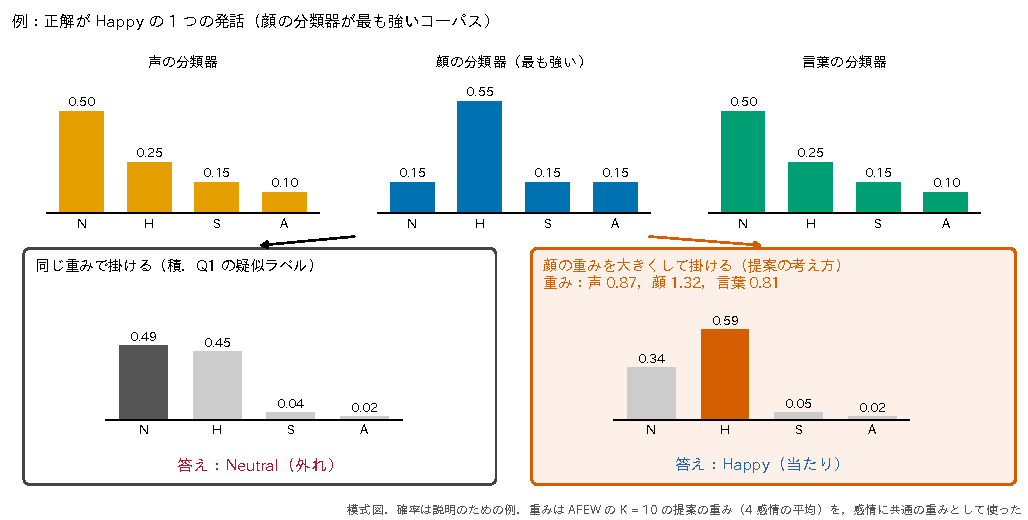
\includegraphics[width=\linewidth,height=0.46\textheight,keepaspectratio]{figures/fig_fusion_example_ja.pdf}
\par\vspace{0.1em}\scriptsize\raggedright
これまでの疑似ラベル（\key{積}）は，3 つの分類器の確率を同じ重みで掛けて作った．上の例（確率は説明用の値）では，本当の感情は Happy で，顔の分類器だけが Happy に高い確率を付けた．同じ重みで掛けると声と言葉の答え（Neutral）に引っ張られて外れ，顔の重みを大きくすると当たる．\par\smallskip
実際の AFEW（K = 5）では，顔の分類器の UAR は \N{usVAFEWfive}\% で，声（\N{usAAFEWfive}\%）と言葉（\N{usTAFEWfive}\%）よりずっと高かった．積でまとめた答えの UAR は \N{uprodAFEWfive}\% で，顔の分類器 1 つより低かった．UAR は 4 感情それぞれの正解率の平均で，当てずっぽうなら 25\% である．
\end{frame}

\begin{frame}{どの分類器が強いかは，コーパスと感情ごとに違う}
\centering
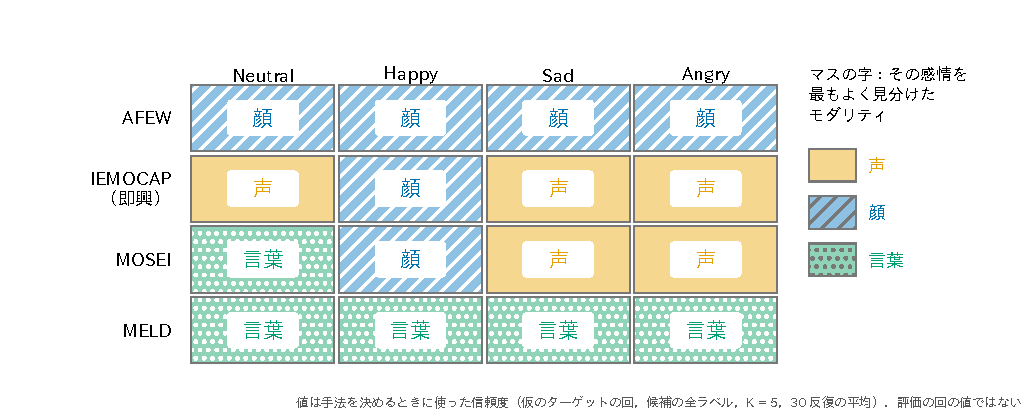
\includegraphics[width=\linewidth,height=0.55\textheight,keepaspectratio]{figures/fig_prop_idea_ja.pdf}
\par\raggedright\scriptsize
各マスは，その感情を最もよく見分けた分類器である（見分ける度合いは後で説明する信頼度 d で測った）．AFEW では 4 感情とも顔，MELD では 4 感情とも言葉だった．IEMOCAP では Happy だけ顔で，ほかは声だった．\par\smallskip
\textbf{提案の考え方}：ターゲットのコーパスごとに，強い分類器の答えを重く数えてからまとめる．得意な感情も分類器ごとに違うので，重みは「分類器 3 つ × 感情 4 つ」の 12 マスの表にする．
\fnote{値は手法を決めるときに使った信頼度（評価に使うコーパスとは別の回．候補の全ラベル，K = 5，30 反復の平均）．評価の回の値ではない．}
\end{frame}

%% =====================================================================
\section{質問 1：12 個の重みは何の重みで，どう使うか}

\begin{frame}{12 個の重みは，分類器が感情に付けた点に掛ける数である}
\ask{12 個の重みは何の重みか．}
\scriptsize
\begin{itemize}\setlength\itemsep{2pt}
\item 重みの表の 1 マス W(分類器, 感情) は，\textbf{その分類器がその感情に付けた点 z に掛ける数}である．表は 3 つの分類器 × 4 つの感情で 12 マスある．
\item \textbf{点 z の定義}：分類器が出した 4 感情の確率の対数から，その 4 つの平均を引いた値（中心化した対数確率）．例えば確率が Happy 0.55，ほかの 3 つが 0.15 なら，z は Happy が +0.97，ほかの 3 つが $-$0.32 になる．
\item 分類器の中の重み（特徴に掛ける数）ではない．3 つの分類器そのものは変えず，出てきた答えのまとめ方だけを変える．
\item 表はターゲットのコーパスと K ごとに 1 つ作り，そのコーパスのすべての発話に同じ表を使う．発話ごとには変えない．
\item 12 個の平均が 1 になるように割る．12 マスがすべて 1 なら，まとめた答えは積と同じになる．1 より大きいマスは，その分類器のその感情の点を積より重く数える．
\end{itemize}
\vspace{-0.4em}\[
s(\text{感情 } i) \;=\; W(\text{声}, i)\, z_{\text{声}}(i) \;+\; W(\text{顔}, i)\, z_{\text{顔}}(i) \;+\; W(\text{言葉}, i)\, z_{\text{言葉}}(i)
\]
\fnote{z の数値の例は計算の説明のための値．log 0.55 − 平均 = +0.97，log 0.15 − 平均 = −0.32（自然対数）．}
\end{frame}

\begin{frame}{重みの表の使い方（1）：点を足し，切片をずらし，疑似ラベルにする}
\ask{12 個の重みをどう使うか．}
\footnotesize
1 つのラベル無しの発話について，次の順に計算する．
\begin{enumerate}\setlength\itemsep{5pt}
\item 3 つの分類器の点 z に，感情ごとに表の重みを掛けて足し，4 つの感情の点 s を出す（前のページの式）．
\item ラベルを使わずに，感情ごとに一定の数（切片 c）を足す．c は，ラベル無しの発話全体で見た各感情の確率の平均が，積の場合の平均と同じになるように決める．答えが 1 つの感情に偏るのを防ぐためである．
\item s ＋ c を softmax で確率に直した q を，その発話の疑似ラベルにする．q は 4 感情の確率のまま使う（柔らかいラベル）．
\item K 本の正解と全部の発話の疑似ラベルで AVT を学び直す．
\end{enumerate}
\vspace{0.4em}
成績は 2 か所で測る．テストの発話で q の最も大きい感情をそのまま答えにしたものを「\key{まとめた答え}」と呼び，学び直す前の成績とする．4 で学び直した AVT の成績も測る．
\end{frame}

\begin{frame}{重みの表の使い方（2）：数値の例}
\centering
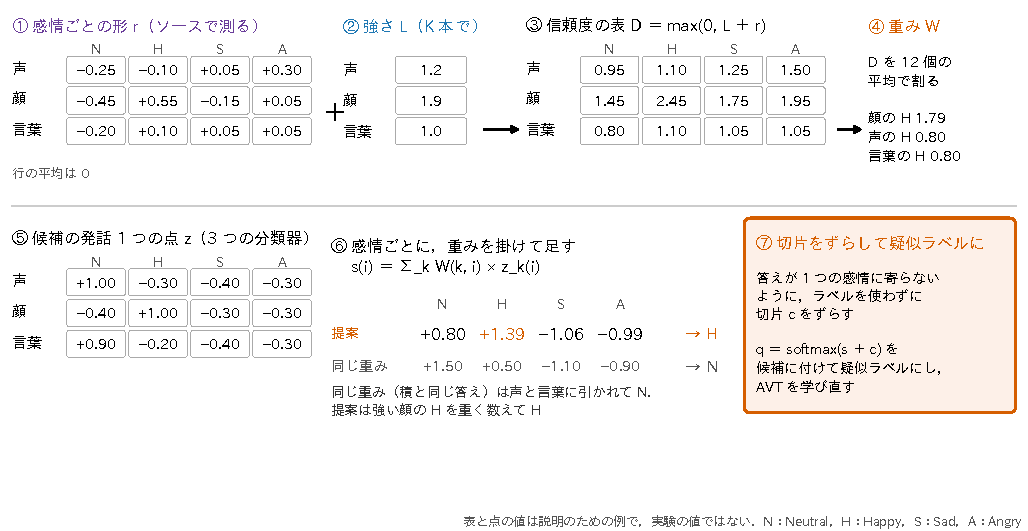
\includegraphics[width=\linewidth,height=0.74\textheight,keepaspectratio]{figures/fig_prop_table_ja.pdf}
\fnote{図の表と点の値は説明のための例で，実験の値ではない．①〜④ は表の作り方（質問 2 で説明する），⑤〜⑦ は前のページの 1〜3 にあたる．}
\end{frame}

\begin{frame}{実際の重みの表（評価の回，K = 10，50 反復の平均）}
\centering
\begin{columns}[T]
\begin{column}{0.48\linewidth}\centering
\wtab{AFEWonezero}{AFEW}\par\vspace{0.6em}
\wtab{MOSEIonezero}{MOSEI}
\end{column}
\begin{column}{0.48\linewidth}\centering
\wtab{IEMOCAPonezero}{IEMOCAP（即興）}\par\vspace{0.6em}
\wtab{MELDonezero}{MELD}
\end{column}
\end{columns}
\par\vspace{0.5em}\scriptsize\raggedright
各表の 12 個の平均は 1 である．右端の「平均」は分類器ごとの 4 マスの平均で，その分類器を全体としてどれだけ重く数えたかを表す．AFEW では顔の行が 4 感情とも大きい（平均 \N{wmeanAFEWonezeroV}）．MOSEI では，顔の Happy（\N{wMOSEIonezeroVH}）と声の Angry（\N{wMOSEIonezeroAA}）が大きく，強い分類器が感情ごとに入れ替わる．
\fnote{N：Neutral，H：Happy，S：Sad，A：Angry．K = 5 と 25 の表は補足に置いた．}
\end{frame}

%% =====================================================================
\section{質問 2：信頼度 d をどう使うか}

\begin{frame}{信頼度 d：分類器がある感情をどれだけ見分けるかの目盛り}
\ask{d をどう使うか（まず d の測り方）．}
\centering
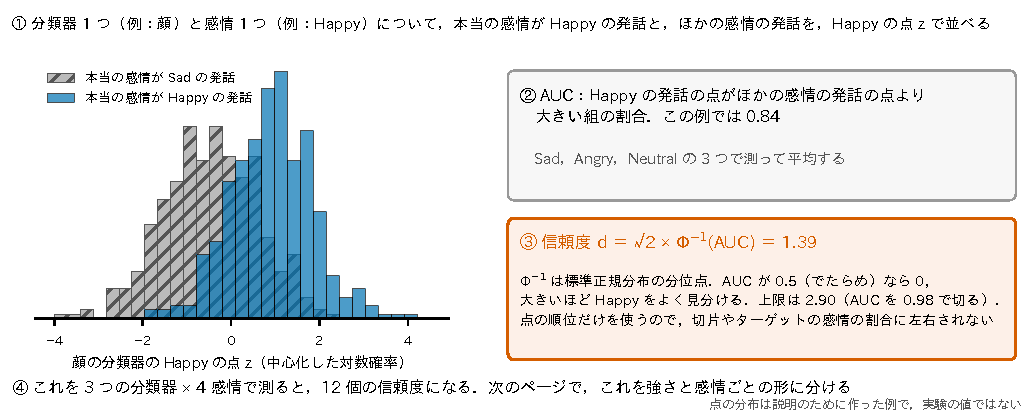
\includegraphics[width=\linewidth,height=0.50\textheight,keepaspectratio]{figures/fig_prop_reliability_ja.pdf}
\par\scriptsize\raggedright
本当の感情が Happy の発話とほかの感情の発話を 1 つずつ組にし，分類器の Happy の点が Happy の発話のほうで高い組の割合（AUC）を数える．d は AUC を「当てずっぽうなら 0，よく見分けるほど大きい」目盛りに直した値である．点の大小だけで決まるので，分類器が特定の感情を多めに答える癖に左右されない．\fnote{図の数値は説明のために作った例．図の AUC 0.84 は丸めた値で，d の 1.39 は丸める前の AUC（0.837）から計算した．}
\end{frame}

\begin{frame}{d は 2 か所で測り，1 つの重みの表に組み立てる}
\ask{d をどう使うか（d から重みへ）．}
\centering
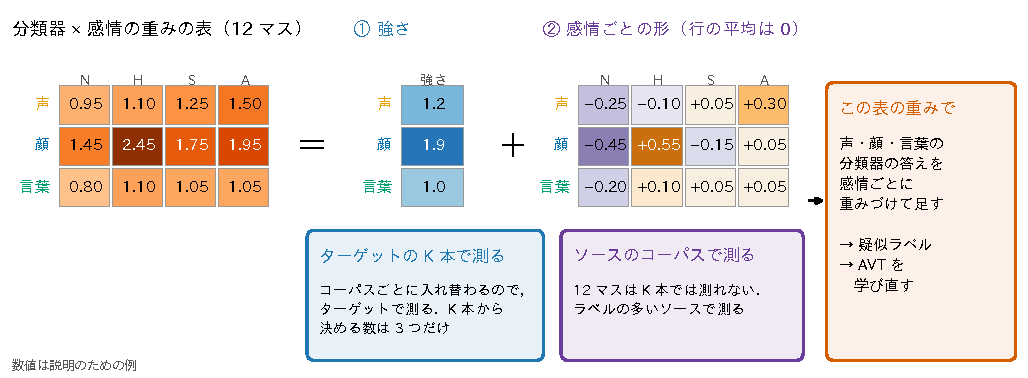
\includegraphics[width=\linewidth,height=0.38\textheight,keepaspectratio]{figures/fig_prop_decomp_ja.pdf}
\par\vspace{0.1em}\scriptsize\raggedright
d は重みの表を作るときだけに使う．テストの発話に答えを付けるときには使わない（図の数値は説明のための例）．
\begin{enumerate}\setlength\itemsep{0pt}
\item \textbf{強さ}（分類器ごとに 1 つ）：ターゲットの K 本で 4 感情の d を測り，平均する．どの分類器が強いかはコーパスごとに入れ替わるので，ターゲットで測る．K 本から決める数は 3 つだけである．
\item \textbf{感情ごとの形}（12 マス）：ラベルの多いソースのコーパスで d を測り，分類器ごとに 4 つの平均を引く．20 本では 12 マスを安定して測れないので，ソースで測る．
\item \textbf{表}：d の表 ＝ max(0, 強さ ＋ 形)．\textbf{重み} ＝ d の表 ÷ 12 個の平均．
\end{enumerate}
\end{frame}

\begin{frame}{強さと形の計算の細部}
\centering
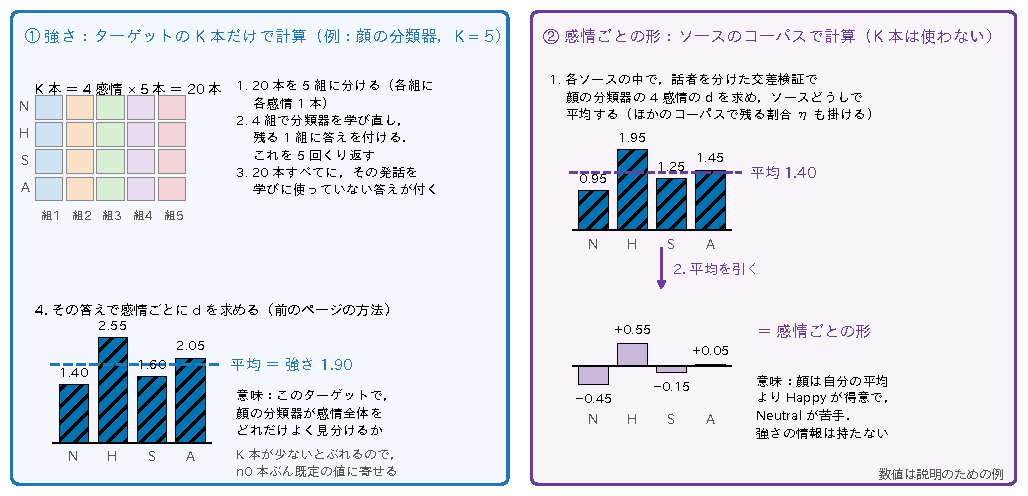
\includegraphics[width=\linewidth,height=0.66\textheight,keepaspectratio]{figures/fig_prop_calc_ja.pdf}
\par\scriptsize\raggedright
強さは，K 本を 5 組に分け，4 組で分類器を学び直して残りの 1 組に答えを付けることを 5 回くり返して測る．学びに使った発話で測ると成績がよく見えすぎるためである．K 本が少ないと強さがぶれるので，n0 本ぶん既定の値に近づける．形は，ソースどうしで別のコーパスに当てたときに d がどれだけ残るか（η）を掛けて弱める．
\end{frame}

\begin{frame}{設定（n0，戻し先，形を使うか）は，評価するコーパスを含まない練習の回で選んだ}
\centering
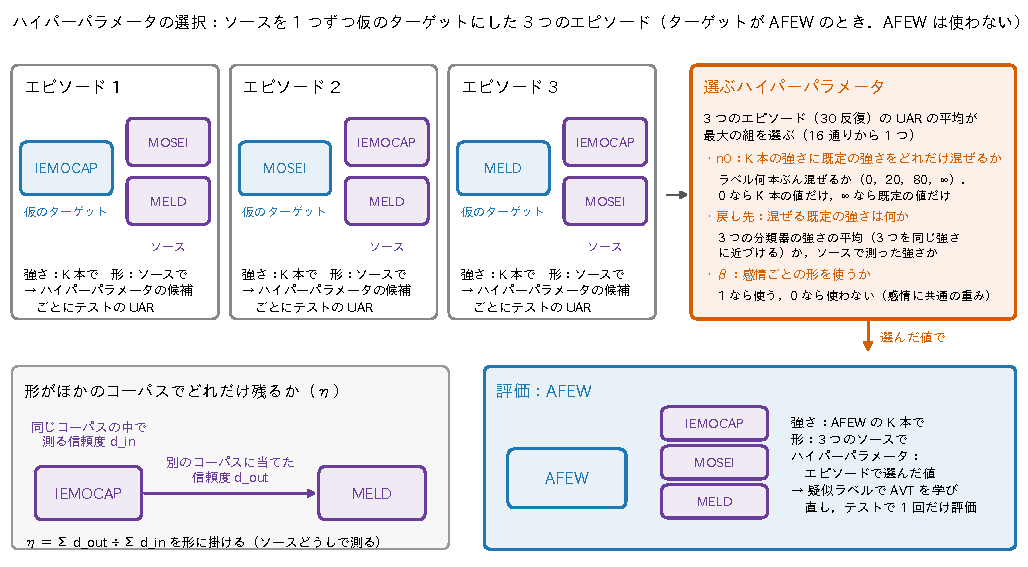
\includegraphics[width=\linewidth,height=0.66\textheight,keepaspectratio]{figures/fig_prop_episode_ja.pdf}
\par\raggedright\fnote{練習の回は，ソースのコーパスを 1 つずつ仮のターゲットにした 3 回（30 反復 ＝ 3 コーパス × 5 分割 × 種 2）．選ばれた値はどの条件でも「形を使う」で，n0 は 12 条件のうち \N{nnzero} で 0 だった．CREMA-D の設定は，元の 4 コーパスを仮のターゲットにした別の下調べで選んだ．手法の形そのものは，評価と同じコーパスの上の下調べで決めた（まとめのページの限界）．}
\end{frame}

%% =====================================================================
\section{質問 3：妥当な比較手法は何か}

\begin{frame}{最も妥当な相手は，同じ 3 つの分類器と同じ K 本でまとめ方だけが違う方法}
\ask{妥当な比較手法は何か．}
\centering
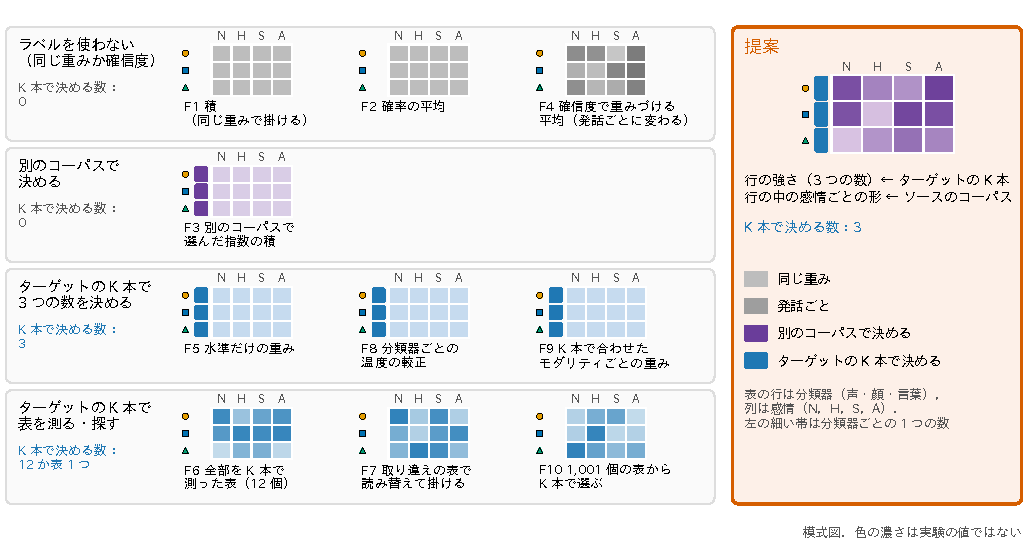
\includegraphics[width=\linewidth,height=0.50\textheight,keepaspectratio]{figures/fig_fusion_glyphs_ja.pdf}
\par\vspace{0.1em}\scriptsize\raggedright
問い 2 は「同じ 3 つの分類器の答えを，まとめ方だけ変えたら，疑似ラベルが当たるようになるか」を問う．そのため最も妥当な相手は，入力（3 つの分類器の確率）と使えるラベル（同じ K 本）が提案と同じで，まとめ方だけが違う方法である．F1〜F10 はどれもこの条件を満たす．
\end{frame}

\begin{frame}{F1〜F10 の群ごとに，提案のどの部分を確かめるか}
\footnotesize
\begin{itemize}\setlength\itemsep{6pt}
\item \textbf{K 本を使わない}（F1 積，F2 確率の平均，F4 確信度で重みづける平均）と\textbf{別のコーパスで決める}（F3 別のコーパスで選んだ指数の積）：K 本で重みを変えること自体が要るか．
\item \textbf{K 本で数個を合わせる}（F5 水準だけの重み，F8 分類器ごとの温度の較正，F9 K 本で合わせたモダリティごとの重み）：感情ごとの形を足すことが要るか．d ではなく尤度で合わせた重みより良いか．F5 は提案から形を外した版である（水準は強さと同じ意味）．
\item \textbf{K 本で表を測る・探す}（F6 全部を K 本で測った表，F7 取り違えの表で読み替えて掛ける，F10 1,001 個の表から K 本で選ぶ）：形を K 本ではなくソースで測ることが要るか．
\end{itemize}
\vspace{0.5em}
F8 は temperature scaling（Guo ほか 2017）を分類器ごとに当てた形，F9 は重みつき対数線形プール（Heskes 1997）の形，F10 はモデル × 感情の重みの乱数探索（Kaya ほか 2017）の形である．F1 は積の規則，F2 は和の規則（Kittler ほか 1998）にあたる．
\end{frame}

\begin{frame}{補助の相手，参照，比べ方の公平さ}
\footnotesize
\begin{itemize}\setlength\itemsep{4pt}
\item \textbf{学び直した 1 つの分類器}：K 本だけで学んだ AVT，積の疑似ラベルで学び直した AVT，温度つき蒸留，一致した発話だけの疑似ラベル，ラベルと疑似ラベルを混ぜる方法，共訓練，共正則化．提案の疑似ラベルで学び直した AVT と比べる．
\item \textbf{標準の手法}（自己学習，エントロピー最小化，情報最大化，T3A，ラベル伝播，CORAL，DANN，MME など）：3 つの分類器の答えを使わない種類の方法なので，UAR を並べるだけにした．
\item \textbf{参照}：同じ形の表を，ターゲットの候補の全ラベルで測った版．実際には使えない．提案の表をどれだけ正確に測れば UAR がどこまで上がるかの目安である．
\item \textbf{公平さ}：どの方法も同じ K 本（同じ引き方），同じテストの発話，同じ 50 反復（分割 5 × K 本の引き方 10）で測った．提案の設定は評価するコーパスを含まない練習の回で選び，F8〜F10 は K 本で合わせた．
\item \textbf{限界}：F3，F5，F6，F7 は，提案の形を選んだ下調べで同じテストの発話の上で見た版である．このため，これらとの差は提案に有利な向きに偏りうる．
\end{itemize}
\end{frame}

%% =====================================================================
\section{質問 4：結果の絶対値}

\begin{frame}{質問 4：結果の UAR の絶対値（\%．差ではなく UAR そのもの．50 反復の平均）}
\centering\tiny\setlength{\tabcolsep}{3.2pt}\renewcommand{\arraystretch}{0.8}
\begin{tabular}{ll|r|rrr|rr|rr|r}\toprule
 & & K 本だけで & \multicolumn{3}{c|}{単独の分類器} & \multicolumn{2}{c|}{まとめた答え} & \multicolumn{2}{c|}{学び直した AVT} & 参照 \\
コーパス & K & 学んだ AVT & 声 & 顔 & 言葉 & 積 & \textbf{提案} & 積の疑似ラベル & \textbf{提案の疑似ラベル} & 全ラベルの表 \\\midrule
\arow{AFEW}{five}{AFEW & 5}\arow{AFEW}{onezero}{ & 10}\arow{AFEW}{twentyfive}{ & 25}\midrule
\arow{IEMOCAP}{five}{IEMOCAP & 5}\arow{IEMOCAP}{onezero}{ & 10}\arow{IEMOCAP}{twentyfive}{ & 25}\midrule
\arow{MOSEI}{five}{MOSEI & 5}\arow{MOSEI}{onezero}{ & 10}\arow{MOSEI}{twentyfive}{ & 25}\midrule
\arow{MELD}{five}{MELD & 5}\arow{MELD}{onezero}{ & 10}\arow{MELD}{twentyfive}{ & 25}\midrule
\arow{CREMAD}{five}{CREMA-D & 5}\arow{CREMAD}{onezero}{ & 10}\arow{CREMAD}{twentyfive}{ & 25}\bottomrule
\end{tabular}
\par\vspace{0.2em}{\tiny\color{mMuted}テストの発話の UAR（当てずっぽうは 25\%）．IEMOCAP は即興の部．CREMA-D は言葉が無いので声と顔の 2 つの分類器をまとめ，K 本だけと学び直しの列は声と顔をつないだ分類器（AV）．単独の分類器はソースで学んだあと K 本で微調整した分類器．参照は実際には使えない．\par}
\end{frame}

\begin{frame}{UAR の絶対値の図}
\centering
\begin{tikzpicture}
\begin{groupplot}[group style={group size=5 by 1, horizontal sep=8mm},
  width=0.235\linewidth, height=0.52\textheight, xmin=0.6, xmax=3.4, xtick={1,2,3}, xticklabels={5,10,25},
  xlabel={K}, tick label style={font=\tiny}, label style={font=\tiny}, title style={font=\scriptsize\bfseries, yshift=-1mm},
  ymajorgrids, grid style={mMuted!25}, every axis plot/.append style={mark size=1.4pt, line width=0.7pt}]
\abspanel{AFEW}{AFEW}\abspanel{IEMOCAP}{IEMOCAP}\abspanel{MOSEI}{MOSEI}\abspanel{MELD}{MELD}\abspanel{CREMAD}{CREMA-D}
\end{groupplot}
\end{tikzpicture}
\par\vspace{0.2em}
{\scriptsize
\textcolor{mMuted}{■} K 本だけで学んだ AVT\quad
\textcolor{mLightBrown}{▲} 積（まとめた答え）\quad
\textcolor{mAccentBlue}{●} 提案（まとめた答え）\quad
\textcolor{mGood}{◆} 提案の疑似ラベルで学び直した AVT\par}
\fnote{縦軸は UAR（\%）．コーパスごとに縦軸の範囲が違う．線は補正しない 95\% 区間（テストの分割と K 本の引き方による揺れから作った）．系列は見やすさのために横に少しずらした．}
\end{frame}

\begin{frame}{絶対値から読めること}
\footnotesize
\begin{itemize}\setlength\itemsep{5pt}
\item \textbf{コーパスごとの水準}：提案のまとめた答えの UAR は，MOSEI で \N{propminMOSEI}〜\N{propmaxMOSEI}\%，MELD で \N{propminMELD}〜\N{propmaxMELD}\%，IEMOCAP で \N{propminIEMOCAP}〜\N{propmaxIEMOCAP}\%，AFEW で \N{propminAFEW}〜\N{propmaxAFEW}\%，CREMA-D で \N{propminCREMAD}〜\N{propmaxCREMAD}\% だった．提案 − 積は AFEW で \N{dppafewmin}〜\N{dppafewmax} 点，ほかの 4 コーパスで \N{dppothmin}〜\N{dppothmax} 点だった．
\item \textbf{K を増やしたときの上がり幅と比べる}：積の UAR は，K を 5 から 25 に増やすと AFEW で \N{prodgainAFEW} 点上がった．AFEW の K = 5 の提案（\N{upropAFEWfive}\%）は，K = 10 の積（\N{uprodAFEWonezero}\%）より高かった．
\item \textbf{参照との差}：同じ形の表を候補の全ラベルで測った参照は，提案より AFEW で \N{orcgapminAFEW}〜\N{orcgapmaxAFEW} 点，IEMOCAP で \N{orcgapminIEMOCAP}〜\N{orcgapmaxIEMOCAP} 点，MOSEI で \N{orcgapminMOSEI}〜\N{orcgapmaxMOSEI} 点，MELD で \N{orcgapminMELD}〜\N{orcgapmaxMELD} 点，CREMA-D で \N{orcgapminCREMAD}〜\N{orcgapmaxCREMAD} 点高かった．AFEW の K = 5 では，参照 − 提案（\N{orcgapmaxAFEW} 点）が提案 − 積（\N{dppAFEWfive} 点）より大きかった．
\item \textbf{K 本だけで学んだ AVT との比べ}：提案の疑似ラベルで学び直した AVT は，4 コーパスの 12 条件のうち \N{nstpropkonly} で K 本だけで学んだ AVT より高かった．IEMOCAP の K = 25（\N{ustpropIEMOCAPtwentyfive} 対 \N{ukonlyIEMOCAPtwentyfive}）と MOSEI の K = 5（\N{ustpropMOSEIfive} 対 \N{ukonlyMOSEIfive}）では低かった．CREMA-D では 3 条件のうち \N{nstpropkonlycremad} で高かった．
\end{itemize}
\fnote{数値はすべて前々ページの表の値から計算した．}
\end{frame}

\begin{frame}{まとめ方の 11 版のうち UAR が最も高かった版（絶対値で見た順位）}
\begin{columns}[T]
\begin{column}{0.56\linewidth}
\centering\tiny\setlength{\tabcolsep}{3pt}\renewcommand{\arraystretch}{0.9}
\begin{tabular}{lllr}\toprule
コーパス & K & 最も高かった版（UAR） & 提案 \\\midrule
\brow{AFEW}{AFEW}\midrule\brow{IEMOCAP}{IEMOCAP}\midrule\brow{MOSEI}{MOSEI}\midrule\brow{MELD}{MELD}\midrule\brow{CREMAD}{CREMA-D}\bottomrule
\end{tabular}
\end{column}
\begin{column}{0.42\linewidth}
\scriptsize\raggedright
提案が 11 版（CREMA-D は F3 が無いので 10 版）の中で最も高かったのは，15 条件のうち \N{ntopprop} だった（MOSEI の 3 つの K と，CREMA-D の K = 5，10）．\par\medskip
AFEW では，K 本で合わせたモダリティごとの重み（F9）が 3 つの K とも最も高く，UAR は提案より \N{fninegapminAFEW}〜\N{fninegapmaxAFEW} 点高かった．差の区間はどれも 0 を含んだ．\par\medskip
提案は積を，AFEW〜MELD の 4 コーパスの 12 条件のうち \N{npppos} で上回った（区間が 0 を含まなかったのは \N{npplo}．CREMA-D を含めると 15 条件のうち \N{nppposall}）．K 本で重みや温度を合わせる方法（F8，F9）との差は，条件によって正にも負にもなった．
\end{column}
\end{columns}
\fnote{11 版のすべての UAR は補足の表に置いた．区間は評価の回の集計（effects.csv）の補正しない 95\% 区間．結果ファイルには派生の版（F9 の切片も合わせる版，F10 の候補を 10 と 100 にした版）もある．これらを含めた 14 版で数えると，AFEW の K = 5 で最も高いのは F9 の切片も合わせる版（\N{tempbAFEWfive}）になり，提案が最も高かった条件の数は \N{ntopproponefour} で変わらない．}
\end{frame}

%% =====================================================================
\section{まとめ}

\begin{frame}{4 つの質問への答え}
\footnotesize
\begin{itemize}\setlength\itemsep{5pt}
\item \textbf{12 個の重みは何の重みで，どう使うか}：声・顔・言葉の分類器がそれぞれの感情に付けた点（中心化した対数確率）に掛ける数である．感情ごとに 3 つの点を重みつきで足し，ラベルを使わずに切片をずらして，疑似ラベル（4 感情の確率）にする．表はコーパスと K ごとに 1 つで，すべてが 1 なら積と同じになる．
\item \textbf{d をどう使うか}：分類器がある感情をどれだけ見分けるかを，順位だけから測った目盛りである．ターゲットの K 本で測った d の平均を分類器ごとの強さに，ソースで測った d の感情ごとの形を 12 マスの形に使い，足して重みの表にする．
\item \textbf{妥当な比較手法}：同じ 3 つの分類器と同じ K 本を使い，まとめ方だけが違う F1〜F10 である．学び直した 1 つの分類器と標準の手法は補助の相手として並べた．
\item \textbf{絶対値}：提案のまとめた答えの UAR は MOSEI の \N{propminMOSEI}\% から CREMA-D の \N{propmaxCREMAD}\% まで，コーパスで大きく違った．提案は積を 4 コーパスの 12 条件のうち \N{npppos} で上回ったが（区間が 0 を含まなかったのは \N{npplo}），11 版の中で最も高かったのは 5 コーパスの 15 条件のうち \N{ntopprop} だった．
\end{itemize}
\fnote{限界：手法の形と設定は，評価に使ったのと同じコーパスの上で作った．テストの発話は，設定を選んだ下調べのテストと同じ発話である．このため，積などとの差は提案に有利な向きに偏りうる．}
\end{frame}

%% =====================================================================
\appendix
\section{補足}

\begin{frame}{補足：まとめ方の 11 版の UAR（K = 5）}
\centering\scriptsize
\begin{tabular}{l|rrrrr}\toprule
版 & AFEW & IEMOCAP & MOSEI & MELD & CREMA-D\\\midrule
\Arow{Fone}{five}{F1 積}\Arow{Ftwo}{five}{F2 確率の平均}\Arow{Fthree}{five}{F3 別のコーパスで選んだ指数の積}\Arow{Ffour}{five}{F4 確信度で重みづける平均}
\Arow{Ffive}{five}{F5 水準だけの重み}\Arow{Fsix}{five}{F6 全部を K 本で測った表}\Arow{Fseven}{five}{F7 取り違えの表で読み替えて掛ける}
\Arow{Feight}{five}{F8 分類器ごとの温度の較正}\Arow{Fnine}{five}{F9 K 本で合わせたモダリティごとの重み}\Arow{Ften}{five}{F10 1,001 個の表から K 本で選ぶ}\midrule
\Arow{prop}{five}{\textbf{提案}}\bottomrule
\end{tabular}
\fnote{まとめた答え（学び直す前）のテストの UAR（\%）．切片をずらした答え．太字は各列で最も高い版．}
\end{frame}

\begin{frame}{補足：まとめ方の 11 版の UAR（K = 10）}
\centering\scriptsize
\begin{tabular}{l|rrrrr}\toprule
版 & AFEW & IEMOCAP & MOSEI & MELD & CREMA-D\\\midrule
\Arow{Fone}{onezero}{F1 積}\Arow{Ftwo}{onezero}{F2 確率の平均}\Arow{Fthree}{onezero}{F3 別のコーパスで選んだ指数の積}\Arow{Ffour}{onezero}{F4 確信度で重みづける平均}
\Arow{Ffive}{onezero}{F5 水準だけの重み}\Arow{Fsix}{onezero}{F6 全部を K 本で測った表}\Arow{Fseven}{onezero}{F7 取り違えの表で読み替えて掛ける}
\Arow{Feight}{onezero}{F8 分類器ごとの温度の較正}\Arow{Fnine}{onezero}{F9 K 本で合わせたモダリティごとの重み}\Arow{Ften}{onezero}{F10 1,001 個の表から K 本で選ぶ}\midrule
\Arow{prop}{onezero}{\textbf{提案}}\bottomrule
\end{tabular}
\fnote{まとめた答え（学び直す前）のテストの UAR（\%）．切片をずらした答え．太字は各列で最も高い版．}
\end{frame}

\begin{frame}{補足：まとめ方の 11 版の UAR（K = 25）}
\centering\scriptsize
\begin{tabular}{l|rrrrr}\toprule
版 & AFEW & IEMOCAP & MOSEI & MELD & CREMA-D\\\midrule
\Arow{Fone}{twentyfive}{F1 積}\Arow{Ftwo}{twentyfive}{F2 確率の平均}\Arow{Fthree}{twentyfive}{F3 別のコーパスで選んだ指数の積}\Arow{Ffour}{twentyfive}{F4 確信度で重みづける平均}
\Arow{Ffive}{twentyfive}{F5 水準だけの重み}\Arow{Fsix}{twentyfive}{F6 全部を K 本で測った表}\Arow{Fseven}{twentyfive}{F7 取り違えの表で読み替えて掛ける}
\Arow{Feight}{twentyfive}{F8 分類器ごとの温度の較正}\Arow{Fnine}{twentyfive}{F9 K 本で合わせたモダリティごとの重み}\Arow{Ften}{twentyfive}{F10 1,001 個の表から K 本で選ぶ}\midrule
\Arow{prop}{twentyfive}{\textbf{提案}}\bottomrule
\end{tabular}
\fnote{まとめた答え（学び直す前）のテストの UAR（\%）．切片をずらした答え．太字は各列で最も高い版．}
\end{frame}

\begin{frame}{補足：実際の重みの表（K = 5）}
\centering
\begin{columns}[T]
\begin{column}{0.48\linewidth}\centering
\wtab{AFEWfive}{AFEW}\par\vspace{0.6em}\wtab{MOSEIfive}{MOSEI}
\end{column}
\begin{column}{0.48\linewidth}\centering
\wtab{IEMOCAPfive}{IEMOCAP（即興）}\par\vspace{0.6em}\wtab{MELDfive}{MELD}
\end{column}
\end{columns}
\fnote{評価の回の 50 反復の平均．各表の 12 個の平均は 1．}
\end{frame}

\begin{frame}{補足：実際の重みの表（K = 25）}
\centering
\begin{columns}[T]
\begin{column}{0.48\linewidth}\centering
\wtab{AFEWtwentyfive}{AFEW}\par\vspace{0.6em}\wtab{MOSEItwentyfive}{MOSEI}
\end{column}
\begin{column}{0.48\linewidth}\centering
\wtab{IEMOCAPtwentyfive}{IEMOCAP（即興）}\par\vspace{0.6em}\wtab{MELDtwentyfive}{MELD}
\end{column}
\end{columns}
\fnote{評価の回の 50 反復の平均．各表の 12 個の平均は 1．}
\end{frame}

\begin{frame}{補足：語と結果ファイルの版の対応}
\centering\scriptsize
\begin{tabular}{ll}\toprule
資料の語 & 結果ファイルの版（\texttt{levels.csv} の \texttt{version}）\\\midrule
提案（まとめた答え） & \texttt{prop} \\
積（まとめた答え） & \texttt{prod} \\
F2〜F10 & \texttt{avg}，\texttt{psel}，\texttt{conf}，\texttt{M\_F2\_K}，\texttt{M\_F6\_K}，\texttt{cf\_D\_l05}，\texttt{tcal}，\texttt{temp}，\texttt{wf1000} \\
単独の分類器（声，顔，言葉） & \texttt{ret\_A}，\texttt{ret\_V}，\texttt{ret\_T} \\
K 本だけで学んだ AVT（CREMA-D は AV） & \texttt{none\_AVT}（\texttt{none\_AV}） \\
積の疑似ラベルで学び直した AVT & \texttt{stud\_prod} \\
提案の疑似ラベルで学び直した AVT & \texttt{stud\_prop} \\
参照：全ラベルで測った表 & \texttt{M\_F6\_orc} \\\bottomrule
\end{tabular}
\par\vspace{0.6em}\raggedright
4 コーパスのまとめた答え・単独の分類器・参照は \texttt{results/dai20\_eval/summary/levels.csv}，学び直した AVT・K 本だけの AVT・CREMA-D は \texttt{results/dai21\_eval5/summary/levels.csv}，重みは \texttt{results/dai20\_eval/summary/weights.csv} の値である（どれも 50 反復，\texttt{seeds = all}）．
\end{frame}

\end{document}
